\RequirePackage{fix-cm}
%
%\documentclass{svjour3}                     % onecolumn (standard format)
%\documentclass[smallcondensed]{svjour3}     % onecolumn (ditto)
\documentclass[smallextended]{svjour3}       % onecolumn (second format)
%\documentclass[twocolumn]{svjour3}          % twocolumn
%
\smartqed  % flush right qed marks, e.g. at end of proof
%
\usepackage{graphicx}
 \usepackage{booktabs}
\usepackage[caption=false]{subfig}
 \usepackage[colorinlistoftodos,backgroundcolor=yellow]{todonotes} %disable
 \usepackage{color}

\usepackage{balance}

\newcommand{\XXX}[1]{\textcolor{red}{{\it \textbf{[XXX: #1]}}}}
\hyphenation{Max-DB data-base}

\usepackage{comment}
\newtheorem{mydef}{definition}
\newcommand{\slbl}[1]{\textbf{\textsf{#1}}}
\usepackage{multirow}%,multicolumn}
\usepackage{slashbox}
\usepackage{wrapfig}
\usepackage{booktabs, colortbl}
\usepackage{amsmath}
\usepackage{url}
\usepackage[pdfstartview=FitH,bookmarksopenlevel=3,bookmarks=true]{hyperref} %pdfpagescrop={92 112 523 778},
\journalname{Empirical Software Engineering}

\begin{document}

\title{Automated Topic Naming}
%\thanks{Grants or other notes
%about the article that should go on the front page should be
%placed here. General acknowledgments should be placed at the end of the article.}

\subtitle{Supporting Cross-project Analysis of Software Maintenance Activities}
%\titlerunning{Short form of title}        % if too long for running head

%\numberofauthors{4}

\author{
Abram Hindle \and
Neil A. Ernst \and
Michael W. Godfrey \and
John Mylopoulos
}
%\authorrunning{Short form of author list} % if too long for running head

\institute{
  Abram Hindle \at 
  Dept. of Computer Science\\
  University of Alberta\\
  Edmonton, AB, CANADA\\
  \email{abram@softwareprocess.es}
\and
  Neil A. Ernst \at
  Dept. of Computer Science\\
  University of British Columbia\\
  Vancouver, BC, CANADA\\
  \email{nernst@cs.ubc.ca}
\and
  Michael W. Godfrey \at
  David Cheriton School of Computer Science\\
  University of Waterloo\\
  Waterloo, Ontario, CANADA\\
  \email{migod@uwaterloo.ca}
\and 
  John Mylopoulos \at
  Dept. Information Eng. and Computer Science\\
  University of Trento\\
  Trento, ITALY\\
  \email{jm@disi.unitn.it}
}

\date{Received: date / Accepted: date}
% The correct dates will be entered by the editor


\maketitle

\begin{abstract}

Researchers have employed a variety of techniques to extract underlying
topics that relate to software development artifacts.  Typically, these
techniques use semi-unsupervised machine-learning algorithms to suggest
candidate word-lists.  However, word-lists are
difficult to 
interpret in the absence of meaningful summary labels.  Current topic modeling 
techniques assume manual labelling and do not use domain-specific knowledge
to improve, contextualize, or describe results for the developers.  
We propose a solution: \emph{automated labelled topic extraction}.
  Topics are extracted 
using  Latent Dirichlet Allocation (LDA) from commit-log comments recovered
from source control systems such as CVS and BitKeeper.  
These topics are given labels from a generalizable
cross-project taxonomy, consisting of non-functional
requirements. Our approach was evaluated with experiments and case studies
on three large-scale Relational Database Management Systems (RDBMS) projects: MySQL, PostgreSQL and MaxDB.  
The case studies
show that labelled topic extraction can produce appropriate,
context-sensitive labels relevant to these projects, which provides fresh
insight into their evolving software development activities.
%160 words
\keywords{ Software maintenance \and Repository mining \and Latent dirichlet allocation \and Topic models}

\end{abstract}

\section{Introduction}
A key problem for practising software maintainers is gaining an
understanding of \emph{why} a system has evolved the way it has. 
This is different from \emph{how} a system has evolved. 
% NE this phrase confuses me: "because the change of behaviour itself is the \emph{how}.
Looking back on streams of artifacts scattered across different
repositories, inferring what activities were performed, when, and for
what reasons, is hard without expert advice from the developers
involved. 
%new stuff
% edit this. awkward
In this work we seek to provide a method of automatically labelling  development topics extracted from commit logs.

Topic modeling is a machine learning technique that creates
multinomial distributions of words extracted from a text corpus. 
This technique infers the hidden structure of a corpus using posterior
inference: the probability of the hidden structure given the data. 
Topic models are useful in software maintenance because they summarize
the key concepts in a corpus, such as source code, commit comments, or
mailing-list messages, by identifying statistically co-occurring words. 
Among other uses, it can quickly give developers an overview of where significant
activity has occurred, and gives managers or maintainers a sense of
project history. 
%A major challenge for topic modeling is to accurately identify the
%summary label for a topic; in the previous case, perhaps
%\emph{``event-handling''} would be appropriate. 
%Current approaches are manual: they rely on human expertise to
%recognize the appropriate label. 
%Furthermore, to date the results of topic modeling are project
%specific, and not generalizable. 
%This paper presents an approach, \emph{labelled topic extraction}, which addresses these two problems.

%migod
While machine learning techniques can automatically identify clumps of
commonly recurring terms, devising an appropriate summary label for
each clump/topic is harder.  
A given topic extracted from a set of commit logs might consist of the following terms: \emph{ ``listener change remove add fire''}. 
This topic might reasonably be labelled as
``\emph{event handling}'' by a developer who understands the domain well,
despite the fact that this label does not appear in the word list itself.  
Current approaches to topic labelling rely on manual intervention by
human experts, and also are limited to project-specific topic labels.  
In this paper, we introduce \emph{labelled topic extraction}, an
approach to topic labelling that creates labels automatically that are
project independent.
%is both automatic and creates labels that are project independent.

% Changes to software systems, revisions, do not occur without
% reason. 
% The reason or purpose is often related to requirements 
% Often one revision might have multiple purposes ranging from
% maintenance issues, quality issues, requirements, features or a
% response to a bug report.
% These purposes often are exhibited as latent topics that relate to
% many development artifacts such as:
%  version control revisions, bug reports, and mailing-list discussions.

%In our previous work we dealt with topic trends, which are topics that recur over time~\cite{Hindle09ICSM}. 
%We observed that topic trends were often non-functional requirements (NFRs). 
%NFRs have the property of being cross-domain and widely applicable. 
%In this sense, they are useful abstractions for developer conversations about different software projects.

% harp on data mining more
%In general, the mining of software artifacts tends to be very project specific, yet NFRs are not. 
% I was told if you're going to use a paren, you don't need to say it.
%There is a series of standards on NFRs, such as ISO9126~\cite{iso9126}, specifically intended to apply to projects of varying types.
%These standards indicate our approach is possible. %, if perhaps not universally accepted).
% NFRs are prevalent in almost all software systems.
% In this paper we will show that NFR related topics occur quite frequently.
%XXXXXX this sentence is confusing
%This informs our method of generalizing the data mining of these software artifacts to leverage the global domain knowledge of software engineering,
%specifically NFRs. 
%In particular, we use software quality models to generalize topics across projects. 
%This allows us to mine software systems with the intention of comparing their NFR-related development topics.
% in order to achieve generalizable, cross project data mining results.

%%%% THIS PARAGRAPH ARGUES ABOUT THE CONCRETE APPLICATION OF 
%%%% TOPIC MODELLING AND LABELLED TOPIC EXTRACTION
%%%% IT NEEDS TO BE TIGHTER BUT IT ALSO NEEDS TO BE HERE

% AH: Topics take a long to read
% AH: Project Dashboards, summarization, software process recovery

%migod
In general, the fruits of mining software artifacts are often project
specific and hard to generalize.  
However, in our previous work we
investigated \emph{topic trends} --- that is, topics that recur over
time --- we observed that topic trends often corresponded to
non-functional requirements (NFRs)~\cite{Hindle09ICSM}, which is
further emphasized in this paper due to the large numbers of NFR
labelled topics.  
This is encouraging, as NFRs have the property of being cross-domain
and widely applicable. 
In this sense, they are useful abstractions for developer
conversations about different software projects.  
Furthermore, there is a series of standards on NFRs, such as ISO9126 \cite{iso9126}, that are specifically intended to apply to projects of varying
types; this suggests that our goal of trying to extract NFR-related development topics, such as those related to software quality models, holds promise.

Concrete applications of topics and \emph{labelled topic extraction}
range from project dashboards to annotating software artifacts such as revisions and bug reports with
NFR-related tags.
Project dashboards~\cite{dashboard} are typically employed by managers and are used to
provide quick summaries of the effort put into a software project. In this case, 
labelled topic extraction would allow managers to track effort
related to NFR topics, such as \emph{portability}.
These techniques also allow for the annotation of commit comments
 and other software artifacts with NFRs. 
This would enable querying of bug reports and artifacts by relevant NFRs. 
For instance a manager can confirm if their developers were
focused on \emph{usability} by looking for
 \emph{usability}-relevant revisions and bug reports.

In this paper, we describe \emph{automated labelled topic extraction}. It addresses two gaps in the topic mining literature:
\begin{enumerate}
  \item Topic mining of software has been limited to one project at a time. 
This is because traditional topic mining techniques are specific to a particular data-set. 
\textit{Automated labelled topic extraction} allows for comparisons \textit{between} projects. 
  \item Topic modeling creates word lists that require interpretation by the user to assign meaning. 
Like (1), this means
that it is difficult to discuss results independent of the project context. 
Our technique automatically, or with some initial training, assigns labels across projects.
\end{enumerate}

This paper makes the following contributions: 
\begin{itemize}
\item introduces the concept of labelled topic extraction, using a non-functional requirements (NFR) taxonomy for our labels; 

%\item evaluates an unsupervised method of automated topic labelling (word-lists);
%%\item Our unsupervised method can be applied to projects without training;
%%\item 
%evaluates a supervised method of automatically labelling topics with a single NFR (machine learning);
%%\item 
%evaluates a supervised method of labelling topics with multiple NFRs
%(multi-label machine learning);

\item evaluates three kinds of automatic topic labelling methods:
  semi-unsupervised labelling  of topics (word-lists), supervised labelling of
  topics with a single NFR (machine learning), 
  and supervised labelling of topics with multiple NFRs (multi-label
  machine learning);

%  of automated topic labelling (word-lists);
%\item Our unsupervised method can be applied to projects without training;
%\item 
%evaluates a supervised method of automatically labelling topics with a single NFR (machine learning);
%\item 
%evaluates a supervised method of labelling topics with multiple NFRs (multi-label machine learning);

\item examines how NFRs correlate with the work of individual developers;
\item provides a method of cross-project analysis via topic labelling; and
 applies these techniques to visualize NFRs over time, and to analyze maintenance activities.

\end{itemize}

%We first introduces labelled topic extraction, and then uses that technique to analyze development activity in two large-scale examples.
We begin by discussing related work in Section \ref{sec:related}.
Next, we describe how we generated our data (Section \ref{sec:wordlist}). For semi-unsupervised classification (Section \ref{sec:unsuplabelling}), we
begin by creating word-lists to signify when a topic matches an NFR label. We then apply our classifier and analyze the results. 
%and how we created the word-lists used in unsupervised classification. 
%We show that labels with their topics can be learned and used to classify other data-sets, either without training 
%Our goal is to label a given topic with either an NFR from our taxonomy,
 %Section \ref{sec:unsuplabelling} presents our technique for using word-lists to do unsupervised classification, and describes the results.
In Section \ref{sec:suplabelling}, we manually annotate the topics, and use those annotations as training data for supervised classification.  
%We then present visualizations of named topics and their trends over time to aid communication and analysis. 
To demonstrate an application of labelled topic extraction, we use an exploratory case study of three open source database systems to show how named
topics can be compared between projects  (Section \ref{sec:analysis}). 
The paper concludes with a discussion of limitations (Section \ref{sec:limit}), and future work.

\section{Previous Work}
\label{sec:related}

The idea of extracting higher-level \emph{concerns} and \emph{topics}, also known as
 \emph{concepts}, \emph{aspects} or \emph{requirements},
has been approached from documentation-based and repository-based
perspectives.

Cleland-Huang and her colleagues have investigated mining requirements
documents for non-functional requirements (NFR) (software
qualities)~\cite{Cleland-Huang2006}.  Their approach is similar to
ours, as they mine keywords from NFR catalogues.  They differ from our approach because
they mine requirements documents where as we mine revisions.
%One approach they tried was similar to this one, with keywords mined from NFR catalogues found in their previous work~\cite{chung99}. 
Their approach resulted in a recall of $80\%$ with precision of $57\%$ for the \emph{security} NFR, but could not find a reliable source of keywords for other NFRs. 
Instead, they developed a supervised classifier by using human experts to identify an NFR training set. 
Our research is different because we use a more comprehensive set of terms based on a taxonomy that is an integral part of our framework.
Another difference is that we make cross-project comparisons instead of focusing
on a single project.
%They relied on requirements documents instead of version control
%histories that we use.
%The objective of Cleland-Huang's study was to identify new NFRs for system development, 
%yet our objective was to recover those latent NFRs from commit-log messages of the project. 

%There are several reasons we did not follow this route. 
%One, we believe we have a more comprehensive set of terms due to the taxonomy we chose. 
%Secondly, we wanted to compare across projects. 
%Their technique was not compared across different projects and the applicability of the training set to different corpora is unclear. 
%A common taxonomy allows us to make cross-project comparison. 
%Although subject to the assumption that all projects conceive of these terms in the same way.
%Thirdly, while the objective of Cleland-Huang's study was to identify new NFRs (for system development) 
%our study assumes these NFRs are latent in the commit-log messages of the project. 

Similarly, Mockus and Votta~\cite{Mockus00} study a large-scale industrial change-tracking system. 
Mockus and Votta leverage WordNet~\cite{Fellbaum1998}, an English-language ``lexical database'' that contains semantic relations between words,
including common related forms (similar to word stemming), meronymy and synonymy.
They use WordNet for word roots as they felt the synonyms would be
non-specific and cause errors.
%, problems we also encountered. 
Mockus et al. validate their labels with system developers.
Since we study multiple projects, instead of a single project, these
kind of interviews are not feasible (particularly in the distributed world of open-source software).

Another approach is to extract concerns from software repositories.
Marcus et al.~\cite{marcus04wcre} use Latent Semantic Indexing (LSI)
to identify commonly occurring concerns for software maintenance. 
The
concerns are given by the user, and LSI is used to retrieve them from
a corpus. 
Topic modelling generates topics that are independent of a user query, and relate only to word frequencies in the corpus.
%Some results were interesting, but their precision was quite low. 
With ConcernLines, Treude et al.~\cite{treude09cl} show tag occurrence
using colour and intensity. 
They mine
developer created tags 
%change request tags (such as `milestone 3') and used these 
in order to analyze the evolution of a single product.
% make evolutionary analyses of a single product. 
The presence of a well-maintained set of tags is obviously essential to the success of this technique.

%XXXXXXXXXXXX OPTIONAL
% Not sure we need this
%Mens et al.~\cite{mens08icsm} conducted an empirical study of Eclipse, a popular Java IDE, to verify the claims of Lehman~\cite{lehman97sms}.
% They concerned themselves with source code only, and found Law Seven, ``Declining Quality'', to be too difficult to assess:
% ``[we lacked an] appropriate measurement of the evolving quality of the system as perceived by the users \cite[p. 388]{mens08icsm}''. 
%This paper examines the notions of quality in terms of a consistent ontology, as Menset al. call for in their conclusions.

% in our previous work~\cite{Hindle09ICSM}, as well as -- CITED a little too often (vanity cites!)
In Baldi et al.~\cite{Baldi2008}, topics are named manually: human
experts read the highest-frequency members of a topic and assign a
label accordingly. 
%XXX Possible to cut this
As discussed earlier, given the topic \emph{``listener change remove add fire''}, Baldi et al. would assign the label \emph{event-handling}. 
The labels are reasonable enough, but still require an expert in the field to determine them. 
Furthermore, these labels are project-specific, because they are generated from the data of that project. E.g., we might have a label called \emph{`Oracle'}
in the MySQL case, since Oracle owns MySQL. 
%We do this differently.
%This paper does this differently. 
Our approach differs: first of all, we automate the process of naming the topics; secondly, we label topics with project-independent terms, in order
to permit cross-project comparison.

Mei et al.~\cite{Mei2007} use context information to automatically name topics. 
They describe probabilistic labelling, using the frequency distribution of words in a topic to create a meaningful phrase. 
They do not use external domain-specific information as we do, but we
do not generate phrases from the topics.

Finally, in Ernst et al.~\cite{ernst10refsq}, we describe our earlier
project, similar to this, that identifies changes in quality requirements
in GNOME software projects; this approach was more exploratory, had
less validation, uses different word-lists, solely uses text-matching,
and does not leverage machine learning strategies. 
Hindle et al.~\cite{Hindle09ICSM} propose a windowed method of topic
analysis that we extend with labelled
topics, NFRs and new visualizations.

%Massey~\cite{massey02icse} and Scacchi~\cite{scacchi02,scacchi05b} looked at the topic of requirements in open-source software. 
% this reduces the line length and drops a ref even though we still have a scacchi kickin around
Massey~\cite{massey02icse} and Scacchi~\cite{scacchi05b} looked at the topic of requirements in open-source software. 
Their work discusses the source of the requirements and how they are used in the development process. 
 German~\cite{german03gnome} looked at GNOME specifically, and listed several sources for requirements: leader interest, mimicry, brainstorming, and prototypes. 
None of this work  addressed quality requirements in OSS, nor did it examine requirements trends.
% NE 0113 this seems too early to mention 'result'.
% Hindle et al. \cite{Hindle2007} examined release patterns in OSS. They showed that there is a difference between projects regarding maintenance
% techniques. This supports our result that software qualities are not discussed with the same frequency across projects.


\section{Study Design and Execution}
Figure \ref{fig:process} gives an outline of our methodology.
We begin by gathering source data and creating topic models. For semi-unsupervised labelling, we generate three sets of word-lists as signifiers for NFRs.
%e created labels using a well-known NFR taxonomy. 
With supervised learning, we train our data with manual annotations in order to match topics with NFRs. Finally, these topics are used to analyze the
role of NFRs in software maintenance.

\begin{figure}
  \centering
 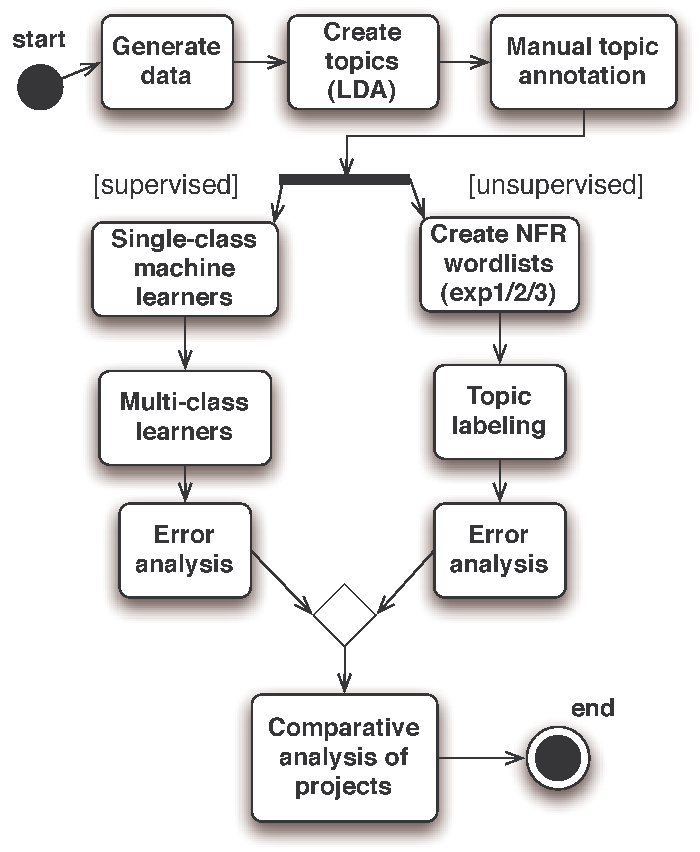
\includegraphics[width=.45\textwidth]{figures/process-model}
 \caption{Research methodology process view.}
  \label{fig:process}
\end{figure}

\subsection{Generating the Data}
\label{sec:wordlist}

To evaluate our approach, we sought candidate systems that were mature projects and had openly accessible source control repositories. 
We selected systems from the same application domain, to control for differences in functional, rather than non-functional, requirements. 
We used three different open-source, partially-commercial database systems:
\begin{itemize}
\item  MySQL 3.23. Started in 1994 and MySQL 3.23 was released in early 2001. MySQL contains $320,000$ lines of C and C++ source code\footnote{generated
using David A. Wheeler's \emph{SLOCCount}, {http://dwheeler.com/sloccount}.}.
\item MaxDB 7.500. Started in the late 1970s as a research project, and was later acquired by SAP. As of version 7.500, released April 2007, the project
has over $940,000$ lines of C source code. 
\item PostgreSQL 7.3. Started in the 1980s as a Berkeley research project. PostgreSQL 7.3 contains $306,000$ lines of C code.
\end{itemize}
  
%Choosing an older version of these projects allowed us to focus on projects which have moved further into the maintenance phase of the software life-cycle.
We explicitly chose older versions of mature projects from a stable problem domain to increase the likelihood that we would encounter primarily
maintenance activities in our studies.

For each project, we used source control commit comments, the messages
that programmers write when they commit revisions to a source control
repository. 
Most commits we observed had commit comments.
Commit comments are often studied by researchers, as they are the most readily accessible source of project interactions, and developers are often
required to create them by the repository mechanism (e.g., Git).  Additionally, relying only on commit comments makes our approach more generalizable,
as we do not assume the presence of other artifact corpora.
%This is the most readily accessible source of project interactions for outside researchers, since developers often or always (e.g., Git) write such
%message. Our approach is more generalizable if it does not assume the presence of other corpora. 
%bug trackers and email-list archives were not available for both projects. 
An example of a typical commit message, from MySQL, is: \textit{``history annotate diffs bug fixed (if mysql\-\_real\-\_connect() failed there were
two pointers to malloc'ed strings, with memory corruption on free(), of course)''}. 
We extracted these messages and indexed them by creation time. 
We summarized each message as a word distribution minus stop-words such as ``\emph{the}'' and ``\emph{at}''. 
%Stemming was performed in the later stages of our analysis. % WAS IT?

For the commit message data-sets of each project, we created an XML file that separated commits into 30 day periods. 
%This size of period, 30 days, is smaller than the time between minor
%releases but large enough for there to be sufficient commits to
%analyze
We chose a period size of 30 days as it is smaller than the time between minor releases but large enough for there to be sufficient commits to
analyze~\cite{Hindle09ICSM}. 
For each 30 day period of each project, we input the messages of that period into Latent Dirichlet Allocation (LDA), a topic analysis
algorithm~\cite{Blei2003}, and recorded the topics the algorithm extracted.
%For each project and for each period of messages a project, we input these messages 
%we created `topics' using Latent Dirichlet Allocation, a topic identification algorithm. 

A topic analysis tool such as LDA will try to find $N$ independent
word distributions within the word distributions of all input messages. 
Linear combinations of these $N$ word distributions are meant to represent and recreate the word distributions of any of the original messages. 
These $N$ word distributions effectively form \emph{topics}: cross-cutting collections of words relevant to one or more of our commit messages. 
LDA extracts topics in an unsupervised manner; the algorithm relies
solely on the source data and word distributions of messages, with no human intervention.

In topic analysis a single document, such as a commit message, can be related to multiple topics. 
Representing documents as a mixture of topics maps well to source code repository commits, which often have more than one purpose~\cite{Hindle09ICSM}.  
For this paper, a topic represents a word distribution generated from a group of commit log comments which are related by their content.  
%In this paper a topic is a set of tokens extracted from commit messages found within a project's source control system (SCS).

We applied Blei's LDA implementation~\cite{Blei2003} against the word distributions of these commits, and generated lists of topics per period. 
We set the number of topics to generate to $20$, because past experimentation showed that fewer topics might aggregate multiple unique topics while
any more topics dilutes the results and creates indistinct topics~\cite{Hindle09ICSM}. 
% Furthermore, more than $20$ topics quickly became infeasible for inspection.

\subsubsection{The High-level Labels}

%\noindent \textbf{The high-level labels} --- 

To facilitate cross-project comparison, we used a taxonomy of NFRs. This taxonomy is based on the ISO quality model, ISO9126~\cite{iso9126}. 
ISO9126 describes six high-level NFRs: maintainability, functionality,
portability, efficiency, usability, and reliability.\footnote{While there may be lingering debate in some circles about these terms, an ISO standard
seems like a reasonable starting point for our work.} 
There is some debate about the terms in this model. 
However, ISO9126 is ``an international standard and thus provides an 
internationally accepted terminology for software quality \cite[p. 58]{Boegh2008},'' that is sufficient for the purposes of this research.  
We claim that these NFRs are maintenance concerns (to varying degrees) in all software projects, and are therefore well-suited for comparisons between
projects.

%\noindent \textbf{Creating a validation corpus} --- 

\subsubsection{Creating a Validation Corpus}
To evaluate both semi-unsupervised and supervised classification, we
created a validation set of manually labelled topics. For each project,
 the annotators (the first two authors) annotated each extracted topic in each period with
the six NFR labels listed above.
Annotators did not annotate each other's annotations, but some brief
inspection of annotations was used to confirm that the annotators were
acting similarly.
We looked at each period's topics, and assessed what the data ---
consisting of the frequency-weighted word lists and messages ---
suggested was the label for that topic. 
We were able to pinpoint the appropriate label using auxiliary information as well, such as the actual revisions and files that were related to the
topic being annotated.
For example, for the MaxDB topic consisting of a message ``exit() only
used in non NPTL LINUX Versions'', we tagged that topic
\emph{portability}. 
Given the top-level annotations of \emph{none}, \emph{portability},
\emph{efficiency}, \emph{reliability}, \emph{functionality},
\emph{usability}, and \emph{maintainability}, the annotators annotated each topic
with the relevant label. Sometimes they used finer-grained
annotations that would be aggregated up to one of these higher-level labels.
%We compared against this data-set, but we also used the data-set for our supervised machine learning based topic classification. 
% A topic may have more than one matching keyword. % ok what?

We validate classification performance using the Receiver Operating
Characteristic area-under-curve value~\cite{Fawcett2006861},
abbreviated \emph{ROC}, and the F-measure, which is the harmonic mean of precision and recall, i.e., $2 * (P * R) / (P + R)$. 

ROC values provide a score %, similar to school letter-grades (A is 0.9, C is 0.6),
 reflecting how well a particular learner performed for the given data. 
ROC maps to the more familiar concepts of precision/sensitivity and recall/specificity: it plots the true positive rate (sensitivity) versus the false
positive rate (1 - specificity). 
A perfect learner has a ROC value of $1.0$, reflecting perfect recall and precision. 
A ROC result of $0.5$ would be equivalent to a random learner (that is, issuing as many false positives as true positives). 
The %area under the -- NE confusing to have area again ... and not importantana
ROC of a classifier is equivalent to the probability that the classifier will rank a randomly chosen positive instance higher than a randomly chosen
negative instance.
We consider our labelling classifiers acceptable if they outperform a random classifier (0.5). 

\subsection{Semi-unsupervised Labelling}
\label{sec:unsuplabelling}

In this section we describe how to label topics based on dictionaries
mined from sources external to the projects.


\subsubsection{Generating Word Lists}

%\noindent\textbf{Generating word lists} --- 

In order to automatically label each topic with 
one of the six high-level NFRs,
%an NFR from ISO9126, 
we associate each NFR with a list
of keywords (\emph{word-lists}, in our parlance). These word-lists were determined a priori and were not extracted from the projects themselves.
We intersected the words of the topics and the words of our word-lists.
We ``labelled'' a topic if any of its words matched any of the word-list's words.
A topic could match more than one NFR.
We used several different sets of word-lists for comparison, which we
refer to as \textsf{exp1}, \textsf{exp2}, and \textsf{exp3} in the text which follows. 

Our first word-list set, \textsf{exp1}, was generated using the ontology described in Kayed et al.~\cite{5072519} .
That paper constructs an ontology for software quality measurement using eighty source documents, including research papers and international standards. 
The labels we used:

\begin{quotation}
\small \noindent \textsf{
integrity, security,
interoperability, testability, maintainability, traceability,
accuracy, modifiability, understandability, availability, modularity,
usability, correctness, performance, verifiability, efficiency,
portability, flexibility, reliability.
}
\end{quotation}

Our second word-list, \textsf{exp2}, uses the ISO9126 taxonomy described above (Section \ref{sec:wordlist}) to seed the word-lists.
%We use these qualities later on as classes in supervised labelling. NE confusing the issue here, I think.
The terms from ISO9126 may not capture all words occurring in the topics that are nonetheless associated with one of the NFRs. 
For example, the term ``redundancy'' is one 
we considered to be
relevant to discussion of \emph{reliability}, but is not in the standard. 
We therefore took the NFRs from the ISO9126 and added terms to them.

To construct these expanded word-lists, we used
WordNet~\cite{Fellbaum1998}.
We then added Boehm's software quality model~\cite{Boehm+:1976:ICSE}, and classified his eleven `ilities' into their respective ISO9126 NFRs. 
We did the same for the quality model produced by McCall et al.~\cite{mccall1977}. 
We then did a simple random analysis of mailing list messages from an open source project, KDE. If we judged a given message to contain terms that were
related to one of the NFRs in ISO9126, we added it to our word-list. This allowed us to expand our word-lists with more software-specific terms.
%Finally, we randomly analyzed two mailing lists from another software project to expand our set with domain-specific terms. 
% Less info is probably better here...
%For example, we add the term ``performance'' to the synonyms for \emph{efficiency}, since this term occurs in most mail messages that discuss efficiency.
Table \ref{tbl:wnsig} shows the labels (NFRs) and word-lists we used for matching.

For the third set of word-lists, \textsf{exp3}, we extended the word-lists from \textsf{exp2} using unfiltered WordNet similarity matches. 
Similarity in WordNet means siblings in a hypernym tree. 
We do not include these words here for space considerations (but see the Appendix for our data repository). 
It is not clear the words associated with our labels in \textsf{exp3} are specific enough. For example, the label \emph{maintainability} is associated with
words \emph{ease} and \emph{ownership}. In general, as we proceed from word-list in \textsf{exp1} to that in \textsf{exp3}, our lists become more generic.

\begin{table*}
	\centering
\begin{tabular}{c|p{9cm}}
\toprule
\textbf{Label} & \textbf{Related terms} \\
\midrule
\emph{Maintainability} &
testability changeability analyzability stability maintain maintainable modularity modifiability understandability interdependent dependency encapsulation
decentralized modular\\ \hline
\emph{Functionality} &
security compliance accuracy interoperability suitability functional practicality functionality compliant exploit certificate secured ``buffer overflow''
policy malicious trustworthy vulnerable vulnerability accurate secure vulnerability correctness accuracy\\ \hline
\emph{Portability} &
conformance adaptability replaceability installability portable movableness movability portability specification migration standardized l10n localization
i18n internationalization documentation interoperability transferability\\ \hline
\emph{Efficiency} &
``resource behaviour'' ``time behaviour'' efficient efficiency performance profiled optimize sluggish factor penalty slower faster slow fast optimization\\
\hline
\emph{Usability} &
operability understandability learnability useable usable serviceable usefulness utility useableness usableness serviceableness serviceability usability
gui accessibility menu configure convention standard feature focus ui mouse icons ugly dialog guidelines click default human convention friendly user
screen interface flexibility\\ \hline
\emph{Reliability} &
``fault tolerance'' recoverability maturity reliable dependable responsibleness responsibility reliableness reliability dependableness dependability
resilience integrity stability stable crash bug fails redundancy error failure\\ 
\bottomrule
\end{tabular}
	\caption{NFRs and associated word-lists -- \textsf{exp2}}
	\label{tbl:wnsig}

\end{table*}

\subsubsection{Automatic Labelled Topic Extraction}

%\noindent \textbf{Generating labels automatically} --- 

Using our three word-lists (\textsf{exp1}, \textsf{exp2}, \textsf{exp3}), we labelled our topics with an NFR where there was a match between a word in
the list and the same word somewhere in the distribution of words that constitute the topic.
A \emph{named topic} is a topic with a match. 
\emph{Unnamed topics} occur where there is no such match. 
This may indicate either a lack of precision in the word-lists, or simply that this topic is not associated with non-functional
requirements.
All experiments were run on the datasets for each project (e.g., PostgreSQL, MySQL, MaxDB). LDA
extracted $20$ topics per period for each project.
% Is this good enough
This labelling is \emph{semi-unsupervised} because the corpus is not derived from 
the project being analyzed, and we did not label the project's topics
ourselves for a training set. The motivation behind this technique is that
because most software often addresses similar issues, we can use the 
domain knowledge of software to label relevant topics.


Table \ref{tbl:wordlist} shows how many topics were labelled for MaxDB
and MySQL.



\begin{table}
\centering
% % This data came from running  
% %   python check_validity.py
% %  in src/validate
% % and then running
% % tail -n 5 *maxdb*yes_no*
% % tail -n 5 *mysql*yes_no*
% ok the new way is to run lda_relator
% src/validate/lda_relator_counts.sh
% NOTE THESE WERE THE OLD VALUES
% WHY DID THEY CHANGE???
% DUNNO
%Named topics	& 281 & 125 & 328  \\
%Unnamed topics & 139 & 295 & 92   \\

% these were check_validate
% MaxDB 7.500 & Named Topics   & 305 & 183 & 330 \\
% MaxDB 7.500 & Unnamed Topics & 84  & 206 & 59   \\
% MaxDB 7.500 & Total  Topics  & 389 & 389 & 389 \\
% MySQL 3.23  & Named Topics   & 341 & 202 & 469 \\
% MySQL 3.23  & Unnamed Topics & 245 & 384 & 117 \\
% MySQL 3.23  & Total  Topics  & 586 & 586 & 586 \\

% these are lda relator

% MaxDB 7.500 & Named Topics   & 281 & 125 & 328 \\ % these numbers are
% 				% slightly different solely because
% 				% we're counting empty topics
% 				% maxdb has 80 empty topics
%  & Unnamed Topics & 219  & 375 &  172  \\
%  & Total  Topics  & 500 & 500 & 500 \\
% \midrule
% MySQL 3.23  & Named Topics   & 524 & 273 & 773 \\
%   & Unnamed Topics & 476 & 727 & 227 \\
%   & Total  Topics  & 1000 & 1000 & 1000 \\

\begin{tabular}{l|c|c|c|c}
\toprule
\textbf{Project} & \textbf{Measure} & \textsf{exp1} & \textsf{exp2} & \textsf{exp3} \\
\midrule
% updated for ESE: taken from latest-reports.tar.gz, last five lines of 
% yes_no_report.txt, using pgsqln instead of pgsqla
 MaxDB 7.500 & Named Topics   & 305 & 183 & 330 \\
             & Unnamed Topics & 84  & 206 & 59  \\
             %& Total Topics   & 400 & 400 & 400 \\
\midrule
 MySQL 3.23  & Named Topics   & 341 & 202 & 469 \\
             & Unnamed Topics & 245 & 384 & 117  \\
             %& Total Topics   & 1000 & 1000 & 1000 \\
\midrule
 PgSQL 7.3   & Named Topics   & 639 & 543 & 640 \\
             & Unnamed Topics & 1   & 97  & 0  \\
             %& Total Topics   & 640 & 640 & 640 \\
\bottomrule
\end{tabular}
	\caption{Automatic topic labelling for MaxDB, MySQL and PostgreSQL}
	\label{tbl:wordlist}

\end{table}

%\DONE{this discussion is about which DB? where do the numbers come from?}
For \textsf{exp1} the labels with the most topics
were
\emph{correctness} (182/305/748 topics) and \emph{testability} (121/238/625). 
We did not see many results for \emph{usability} (4/0/138) or
\emph{accuracy} (3/0/27), which were associated with fewer than ten topics. 
We also looked for correlations between our labels: excluding double
matches (self-correlation), our highest co-occurring terms were
\emph{verifiability} or \emph{correctness}
with \emph{traceability}, and \emph{testability} with \emph{correctness} (76 and 62 matches, respectively).
% See the following sections for our error analysis. 



For \textsf{exp2}, there are more unnamed topics than \textsf{exp1}. 
Only \emph{reliability} produces the most matches, mostly due to the word ``error''. 
Co-occurrence results were poor. This suggests our word lists were overly restrictive.
For PostgreSQL \emph{reliability} and  \emph{usability} co-occurred
with \emph{portability} and \emph{efficiency}.


For \textsf{exp3}, we generally labelled more topics. 
As we mentioned, the word-lists are broad, so there are likely to be false-positives (discussed below). 
The most frequent label across all projects was \emph{usability}, and the
least frequent label was \emph{maintainability}. 
Common co-occurrences were \emph{reliability} with \emph{usability}, \emph{efficiency} with \emph{reliability}, and \emph{efficiency} with \emph{usability}.
%(200, 190, and 150 topics in common, respectively). 




\subsubsection{Analysis of the Semi-unsupervised Labelling} %--- %Based
				%on the labels, and our manual topic
				%labelling, 
%\noindent \textbf{Analysis of the unsupervised labelling} --- %Based on the labels, and our manual topic labelling, 
%we compared the results of the unsupervised word matching approach. 
For each quality we assessed whether semi-unsupervised labels matched the manual annotations. 
To be clear, the manual annotations were not used to
train the labelling process.
As described in Section \ref{sec:wordlist} we used both ROC and F-1 measures to evaluate the performance of the classification.
Figure \ref{fig:maxdb-unsup-results} shows our ROC results for PostgreSQL, MaxDB and MySQL. We describe F-1 results in the text below.


% \begin{figure}[t]
% \centering
% \subfloat[ROC]{
%  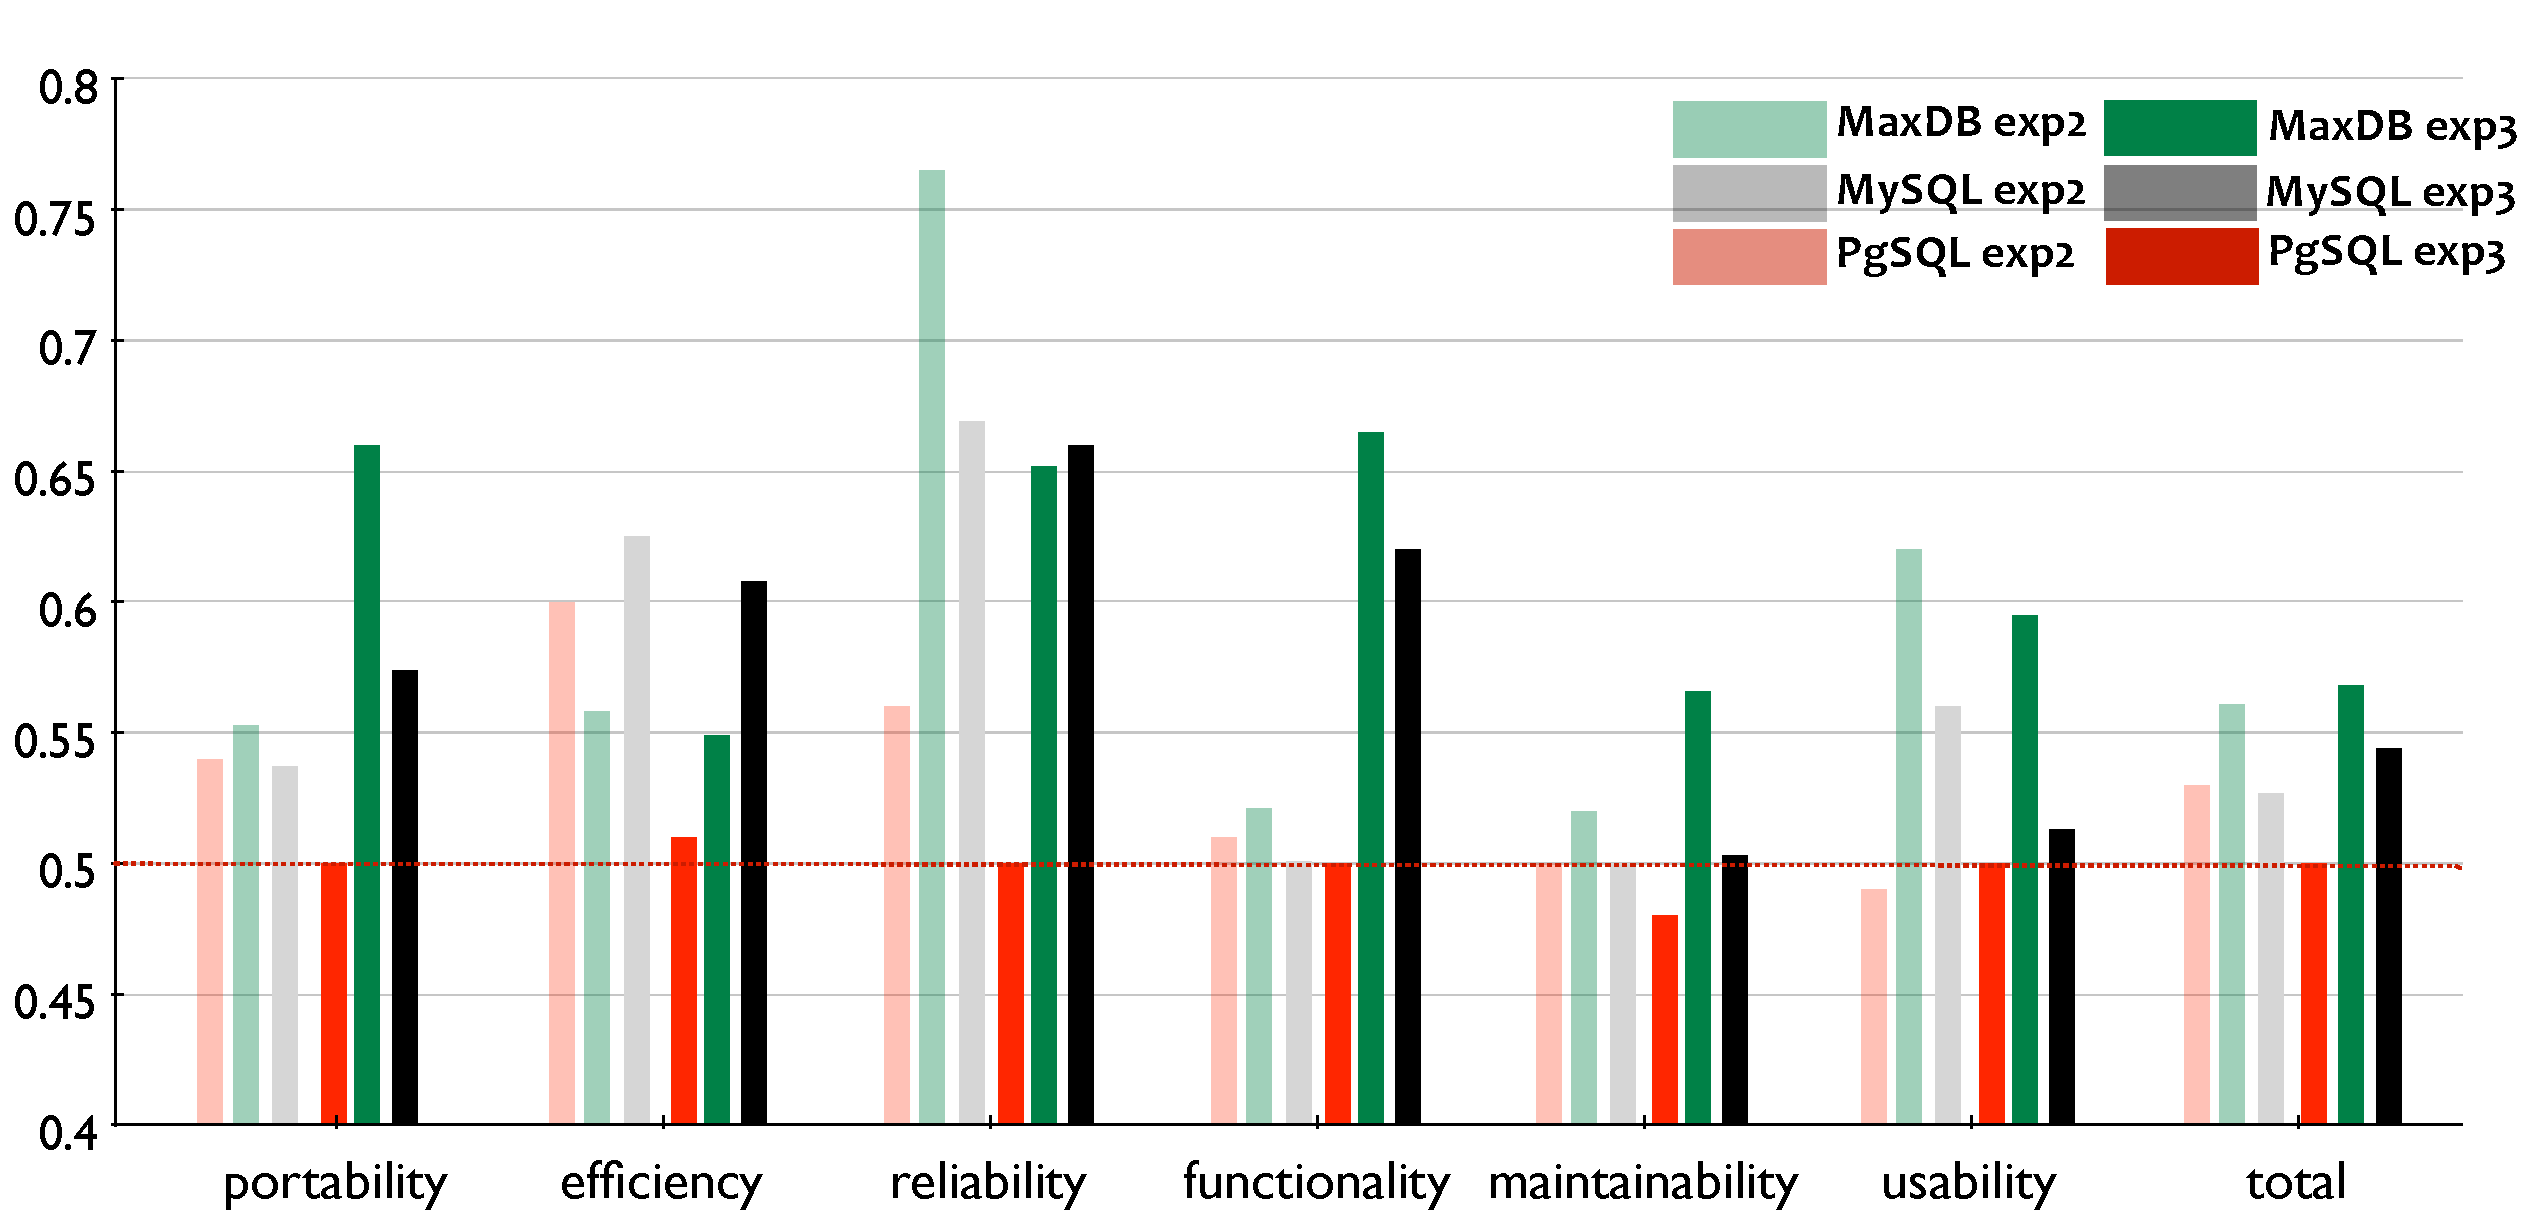
\includegraphics[width=0.45\textwidth]{figures/unsupervised-bar}
% \label{fig:maxdb-unsup-results-roc}
% }
% %\subfloat[F1]{
% %\includegraphics[width=0.45\textwidth]{figures/unsupervised-bar-f1}
% %\label{fig:maxdb-unsup-results-f1}
% %}
% \caption[]{Performance of unsupervised topic labelling for each NFR per word-list. A) ROC values -- 
% dashed line indicates the performance of a random classifier. B) F1 measure. Possible values range from 0--1.

% }
% \label{fig:maxdb-unsup-results}
% \end{figure}


\begin{figure*}[t]
  \centering
 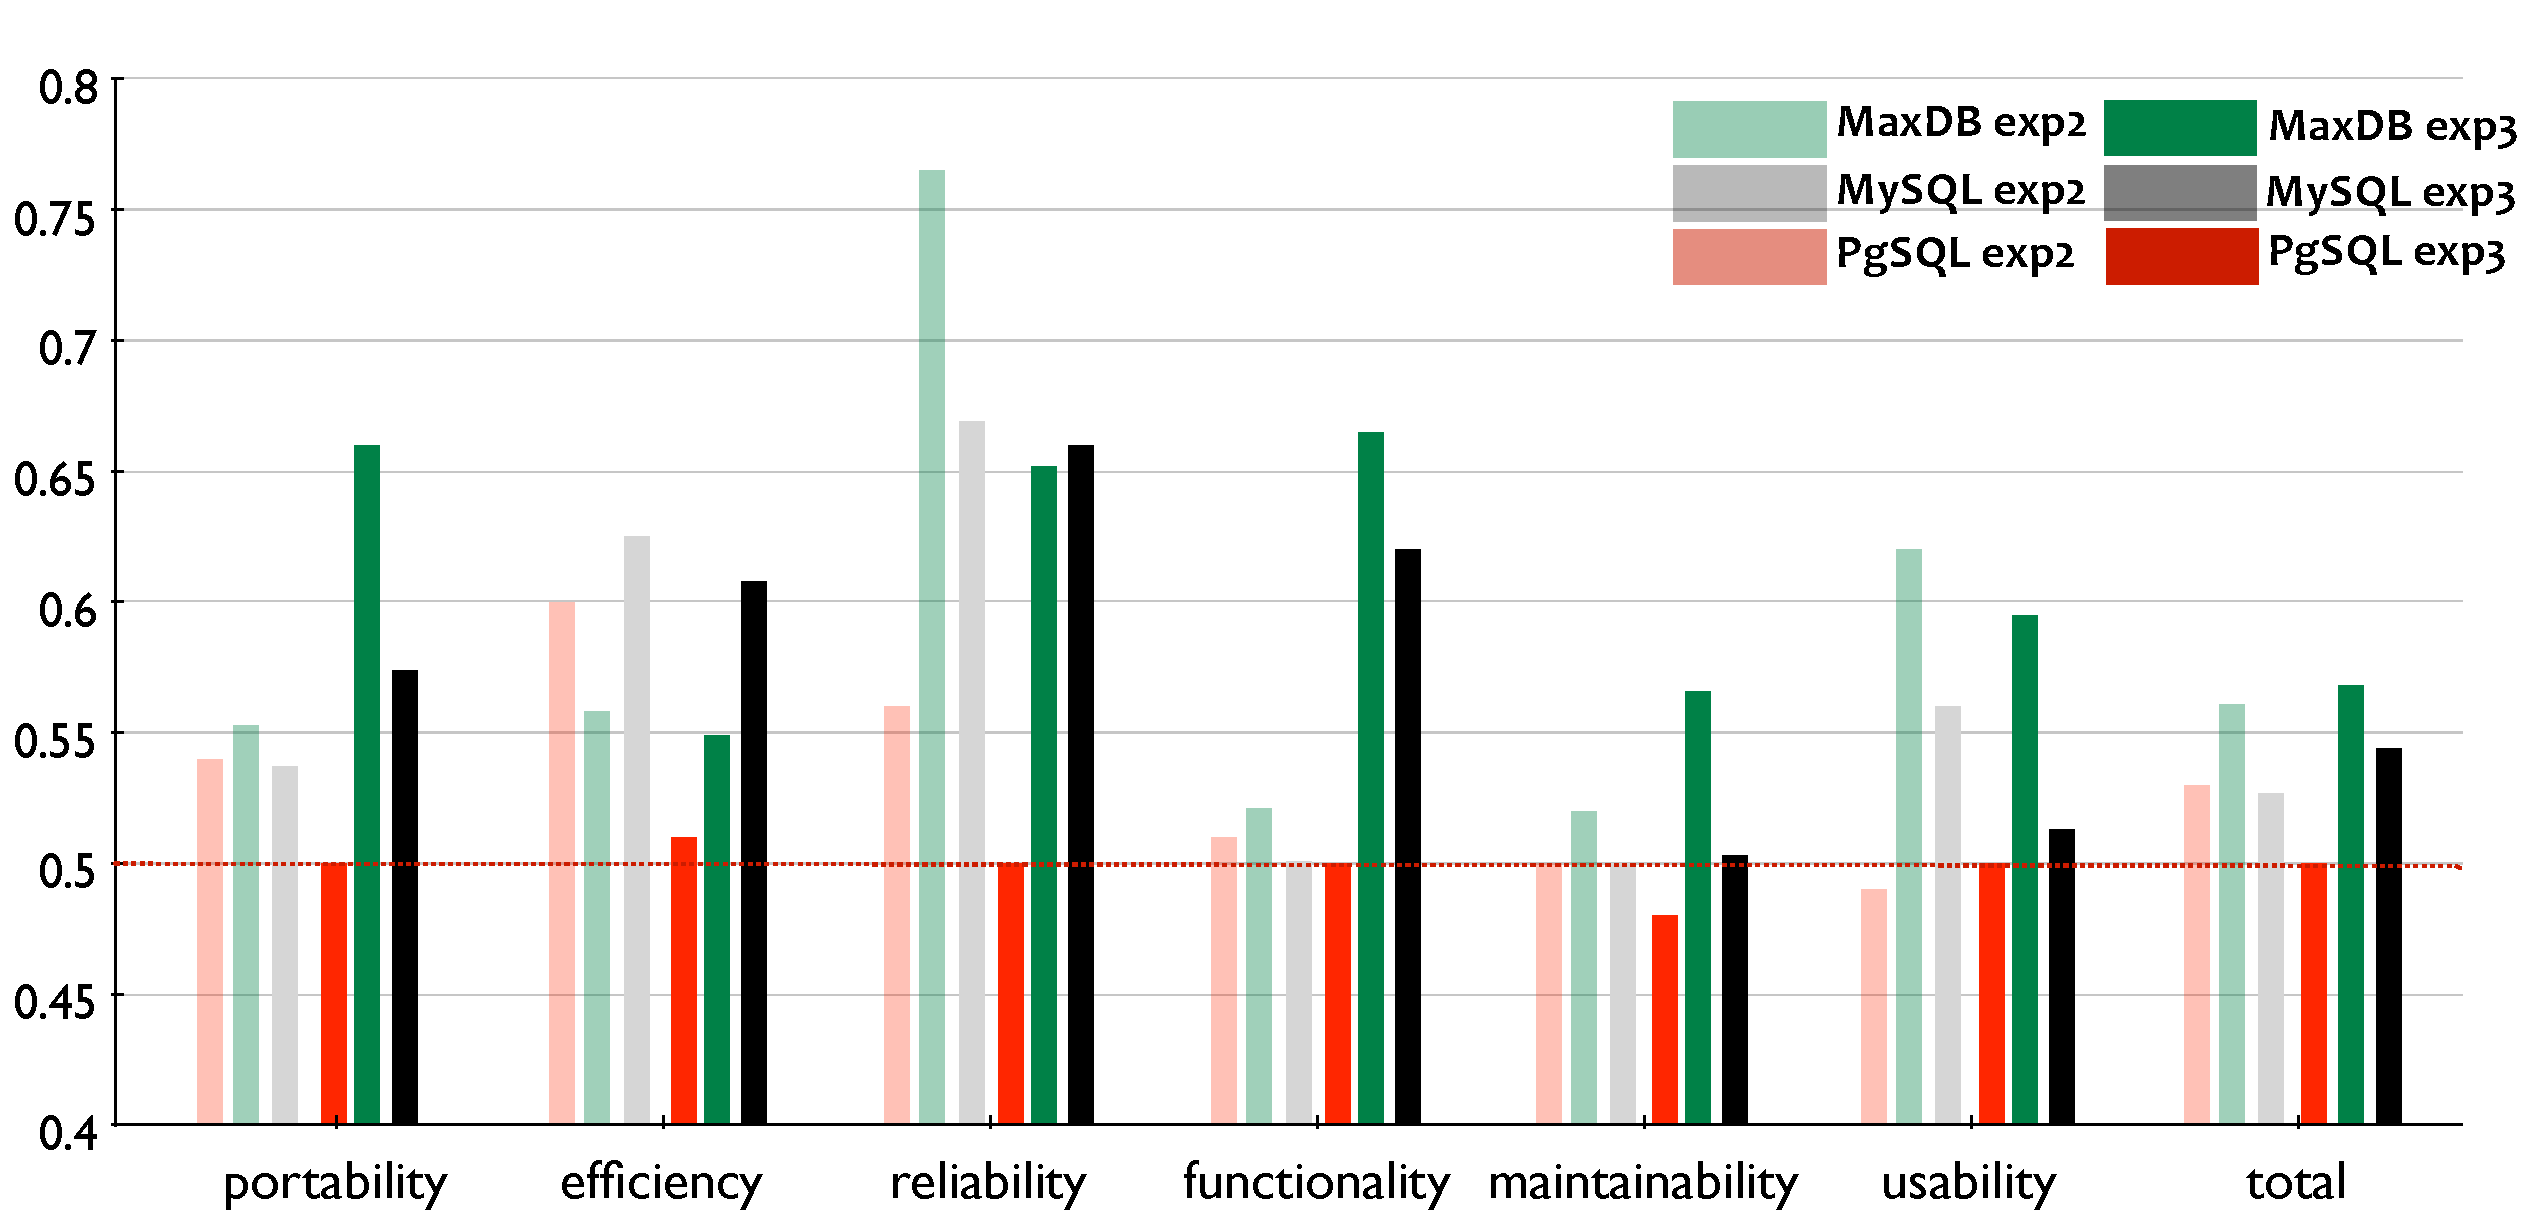
\includegraphics[width=0.8\textwidth]{figures/unsupervised-bar}
 \caption{Performance, ROC values (range: $0$--$1$), of semi-unsupervised topic labelling for
   each NFR and per word-list. The dashed line indicates the performance of a random classifier. This graph shows how well the
   semi-unsupervised topic labelling matched our manual annotations.}


  \label{fig:maxdb-unsup-results}
\end{figure*}


Because our ground truth annotations were relevant only to ISO9126,
we estimate that \textsf{exp1} had poor
performance via the overlap between ISO9126 and the Kayed ontology.
For \textsf{exp1} the F-measures for MaxDB were from $0$ to $0.18$ with an average
of $0.03$, for MySQL were from $0$ to $0.16$ with an average of
$0.05$, and for PostgreSQL $0$ to $0.15$ with an average of $0.07$. 

%\DONE{update these numbers but from where? }
% 0.177215189873 / 6
% .02953586497883333333
% (0.0298507462687 + 0.0661157024793 + 0.0634920634921 + 0 + 0.115384615385) / 6
% .04580718793751666666

% pgsql
% portability 
% 0.0910746812386
% efficiency 
% 0.154639175258
% reliability
% 0.0470588235294
% maintainability
% 0
% usability
% 0.0720720720721
%> v <- c(0.0910746812386 , 0.154639175258 , 0.0470588235294 , 0 , 0.0720720720721)
%> summary(v)
%   Min. 1st Qu.  Median    Mean 3rd Qu.    Max. 
%0.00000 0.04706 0.07207 0.07297 0.09107 0.15460 


% EXP2 source is latest-reports/exp2-unsup-results.xls. Numbers reflect latest runs as of 08/2011.
% (change as needed). Second column (after the name) is F1.
% column format is determined by info-theory.py : accuracy	f1	fn	fp	mcc	precisions	recall	roca	tn	tnr	tp
For \textsf{exp2}, the average F-measure (macro-F1) for MaxDB was  $0.24$ with a range $0.091$ to
$0.37$, and $0.16$ for MySQL with a range of $0$ to $0.41$. PostgreSQL had an average F-measure of $0.30$ %using pgsqln
 with a range of $0.09$ to $0.38$.
MaxDB had an average precision and recall of $0.25$ and $0.22$
while MySQL had $0.41$ and $0.10$ and PostgreSQL $0.31$ and $0.29$, respectively.

% EXP3
For \textsf{exp3}, the average F-measure (macro-F1) for MaxDB was $0.26$ with a range $0.11$ to
$0.47$, and $0.36$ for MySQL with a range of $0.10$ to $0.65$. 
PostgreSQL had an average of $0.42$ with a range of $0.31$ to $0.54$.
MaxDB had an average precision and recall of $0.16$ and $0.67$
while MySQL had $0.3$ and $0.48$. PostgreSQL had precision and recall of $0.27$ and $0.95$, respectively.

Based on this we found that \emph{reliability} and
\emph{usability} worked well for MaxDB in \textsf{exp2} and better in
\textsf{exp3}. 
\textsf{exp1} performed poorly.
MySQL had reasonable results within \textsf{exp2} for \emph{reliability} and \emph{efficiency}. 
MySQL's results for \emph{efficiency} did not improve in \textsf{exp3}
but other qualities such as \emph{functionality} did improve. 
For PostgreSQL in \textsf{exp2}, \emph{reliability} and \emph{efficiency} were likewise the most accurate,
while \emph{functionality} remained poor. \emph{Functionality} improved dramatically by \textsf{exp3}.
Many ROC scores were $0.6$ or less, but our classifier still performed substantially better than random.

%\vspace*{-1em}
\subsection{Supervised Labelling}
\label{sec:suplabelling}
Supervised labelling requires expert analysis of the correct
class/label to assign a label to a topic. In our approach, we use the top-level NFRs in the ISO9126 standard~\cite{iso9126} for our classes, but other
taxonomies are also applicable.%In order to validate how effective these word-bag approaches to topic labelling would be we created a validation data set. 

We used a suite of supervised classifiers, WEKA~\cite{weka09},
that includes machine learning tools such as support vector machines and Bayes-nets. 
We also used the multi-labelling add-on for WEKA, Mulan~\cite{mulan}. %\footnote{\url{http://mlkd.csd.auth.gr/multilabel.html}}. 
Traditional classifiers label topics with a single class, whereas Mulan allows for a mixture of classes per topic, which is what we observed while
manually labelling topics.
The \emph{features} we used are word counts/occurrence	per topic, if
a word occurs frequently enough in a topic we consider it a feature of
the topic.

To assess the performance of the supervised learners, we did a 10-fold cross-validation~\cite{Kohavi1995}, a common technique for evaluating machine
learners. 
The original data is partitioned randomly into ten sub-samples. Each sample is used to test against a training set composed of the nine other samples.
%One subsample is used as a training set and evaluated on the other nine sub-samples. 
%This is repeated nine more times, with each subsample used once as the training set. 
We have reported these results below.% in Section \ref{sec:suplabelling}.

\subsubsection{Analysis of the Supervised Labelling}
% \label{sec:suplabelling}
Because our data-set was of word counts we expected Bayesian techniques, often used in spam filtering, to perform well. 
We tried other learners that WEKA~\cite{weka09} provides: rule learners, decision tree learners, vector space learners, and support vector machines.  
Figure \ref{fig:best-learn-per-tag} shows the performance of the best
performing learner per label: 
% We considered the best learner for a label to be 
the learner that had the highest ROC value for that label. 
The best learner is important because one uses a single learner per
label. When applying our technique, for each NFR one should select the best learner possible.
%Figure \ref{fig:best-learn-per-tag} uses the ZeroR learner as a baseline, a common practice in machine learning,
%as ZeroR naively chooses the largest category all of the time. 
%ZeroR occasionally outperforms other learners; for labels which are not as common, this is to be expected because any miscategorization will hurt accuracy. 
%This is why we use ROC values, instead of accuracy, as they can better represent performance on labels which are not applicable to the majority of samples.

Figure \ref{fig:best-learn-per-tag} shows that MaxDB and MySQL have
quite different results, as the ROC values for \emph{reliability} and
\emph{functionality} swap between projects. For PostgreSQL, the
performance is nearly always more poor than the other two systems. The
reason for this lack of performance could be that the number of
topics, $N$ could be non-optimal for PostgreSQL. Perhaps topics were
getting too mixed and it was becoming hard to distinguish one topic
from the next. PostgreSQL's dataset was the largest of the 3 projects,
the XML data-dump that described the PostgreSQL topics that we
annotated was 8X larger than MySQL and 1.7X larger than MaxDB. These
size differences arise from the number of commits, the number of files
and the verbosity of the commit descriptions.

%\DONE{expand on why?}

% PG data from abram's email of 09/01/2011 using first column and pgsqln.
\begin{figure}[t]
\centering
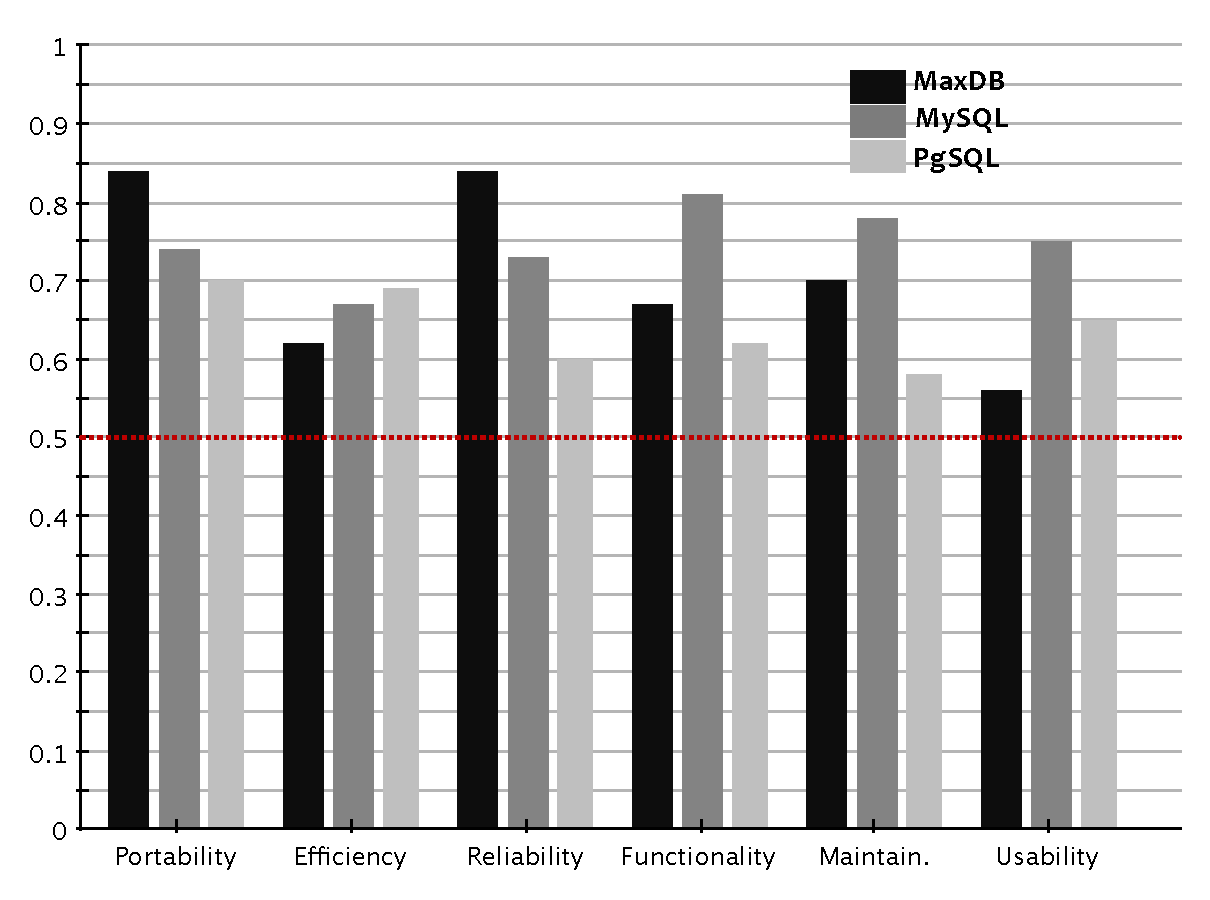
\includegraphics[width=0.45\textwidth]{figures/both-supervised}
\caption[]{ROC value for the best learner per label for MaxDB, MySQL and PgSQL. Values range from $0$--$1$.  Dashed line indicates the performance of a random
classifier.
}
\label{fig:best-learn-per-tag}
\end{figure}

For all projects Bayesian techniques did the best out of a wide variety of machine learners tested. 
Our best learners, Discriminative Multinomial Naive Bayes, Naive Bayes
and Multinomial Naive Bayes  are all based on Bayes' theorem and all
assume, naively, that the features supplied are independent. 
%The features we used are word counts per message. 
One beneficial aspect of this result is that it suggests we can have
very fast training and classifying  since training or classifying one
instance of Naive Bayes can be calculated in $O(N)$
for $N$ features.
%http://nlp.stanford.edu/IR-book/html/htmledition/naive-bayes-text-classification-1.html

% # F measure
% mysql
% > v <- c( 0.64 , 0.23  ,0.41 , 0.77  ,0.62 , 0.21 ) 
% > summary(v)
%    Min. 1st Qu.  Median    Mean 3rd Qu.    Max. 
%   0.210   0.275   0.515   0.480   0.635   0.770 
% maxdb
% > v <- c(0.61, 0.25, 0.59, 0.32, 0.42, 0.17)
% > summary(v)
%    Min. 1st Qu.  Median    Mean 3rd Qu.    Max. 
%  0.1700  0.2675  0.3700  0.3933  0.5475  0.6100 

%src/validate/latex-out/best-learner-per-project-roc
The range of F-measures for MySQL was $0.21$ to $0.77$ with a mean
of $0.48$. MaxDB had a range of $0.17$ to $0.61$ with a mean
of $0.39$. Finally, PostgreSQL had a range of $0.04$ to $0.9$ and a mean of $0.43$.


The less-frequently occurring a label, the harder it is to get accurate
results, due to the high noise level. Nevertheless, these results are
better than our previous word-list results of \textsf{exp2} and
\textsf{exp3}, because the ROC values are sufficiently higher in most
cases (other than MaxDB \emph{reliability}, MySQL \emph{efficiency}, and PgSQL \emph{maintainability}). The
limitation of the approach we took here is that we assume labels are
independent; however, labels could be correlated with each other. 
The next section (\ref{sec:multilabel})
addresses the issue of a lack of independence and correlation between
labels
using multi-label learners.
%In the next section we will evaluate how well these learners perform
%together.
%\todo[inline]{Comment about correlation, we should link to the Mulan section, perfect segway since Mulan relies on correlation.}

%\balance

\subsection{Applying Multiple Labels to Topics}
\label{sec:multilabel}

As noted in Section \ref{sec:wordlist}, each topic in our data-set can be composed of zero, one, or more NFRs. 
For example, a commit message might address \textit{reliability} in the context of \textit{efficiency}, or make a \textit{maintainability} improvement
in the source code that related to \textit{usability}. 
However, traditional machine learning techniques, such as Naive Bayes, can only map topics to a single class. 
The Mulan~\cite{mulan} library encapsulates several different multi-label machine learners which can label elements with multiple labels.
Mulan also includes methods for determining the performance of such techniques.
% TOO DETAILED The problem framed in the learners above has changed; instead of looking at the precision and recall of applying one label, we rank
% multiple labels at once. We must check if the full subset of labels was applied, and then how much of that subset was applied.

% Data source is src/validate/output/<db>.mulan.out.tex
% pgsqln & br & clr & homer
% macro-auc .64 .58 .58
% micro .65 .6 .6
%pgsqla
% macro .63 .56 .54
% micro .81 .81 .79
% maxdb (no macro)
% micro .77 .67 .61
% mysql
% macro .74 .65 .64
% micro .81 .8 .74

\begin{figure*}[t]
\centering
\subfloat[MySQL]{
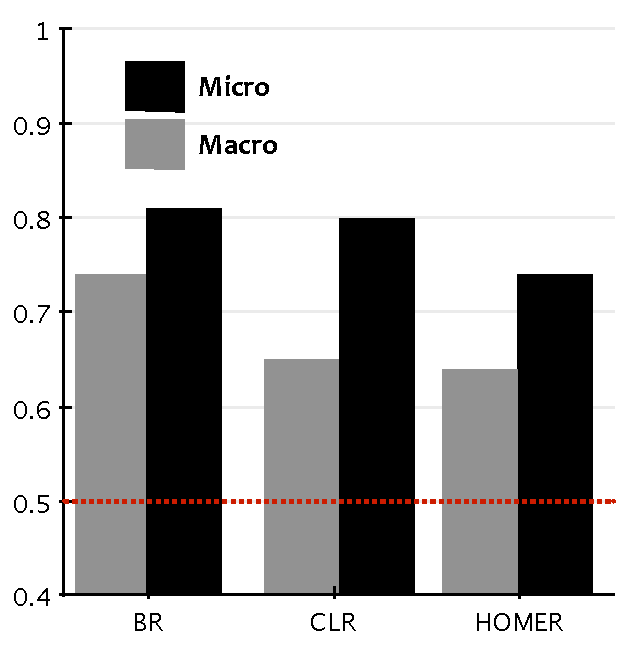
\includegraphics[width=0.4\textwidth]{figures/multi-label-results-mysql}
\label{fig:subfig3}
}
\subfloat[MaxDB]{
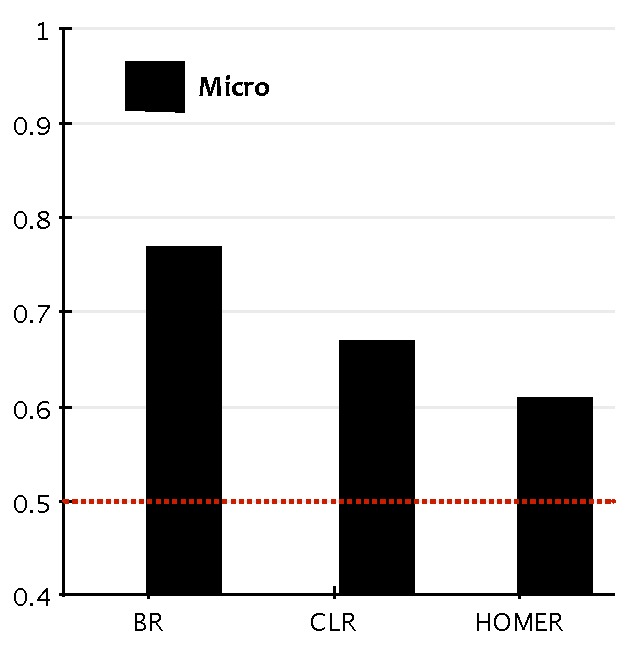
\includegraphics[width=0.4\textwidth]{figures/multi-label-results-maxdb}
\label{fig:subfig4}
}
\caption[]{MySQL and MaxDB macro and micro-ROC results per multi-label learner. Possible values range from $0$--$1$.  Dashed line indicates the performance of a random classifier.
}
\label{fig:mulan}
\end{figure*}

\begin{figure}
\centering
\subfloat[Macro-ROC]{
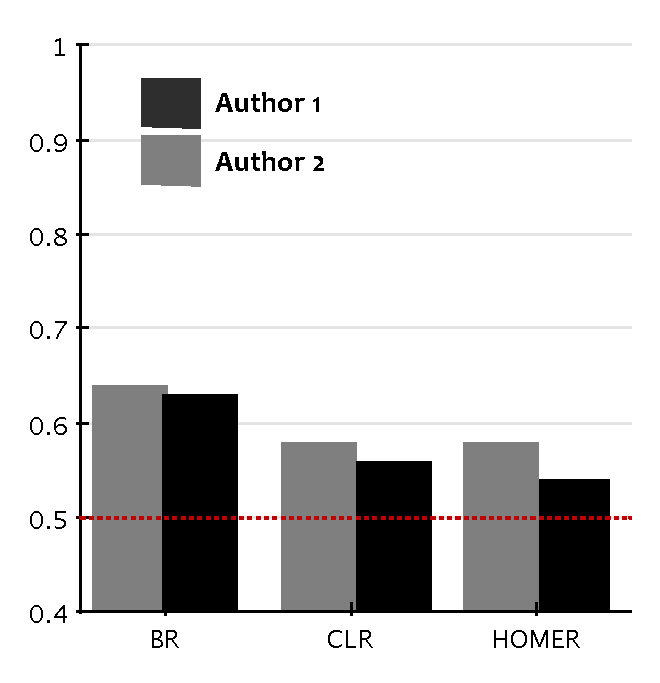
\includegraphics[width=0.4\textwidth]{figures/pg-mulan-macro-compare}
\label{fig:pgcomp-a}
}
\subfloat[Micro-ROC]{
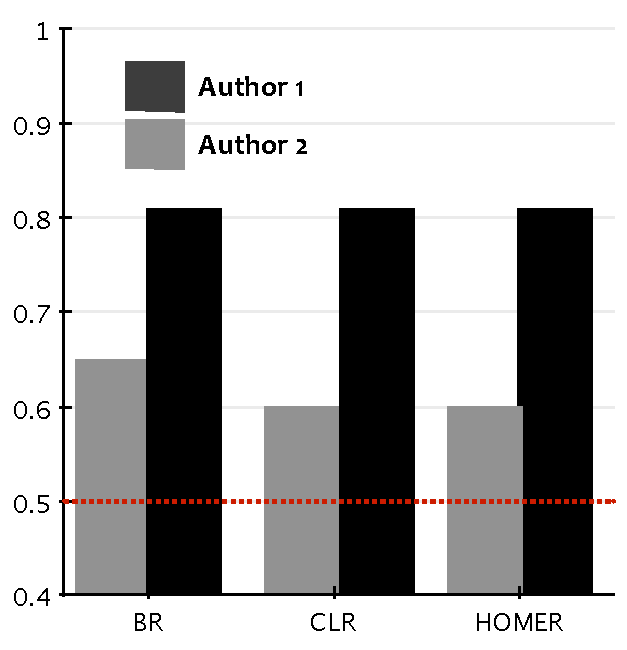
\includegraphics[width=0.4\textwidth]{figures/pg-mulan-micro-compare}
\label{fig:pgcomp-b}
}
\caption{Author \#1 and author \#2 ROC results for PostgreSQL.} 
\label{fig:pgcomp}
\end{figure}

Two perspectives to evaluate multi-label learners are with micro or macro measurements (used in Figure \ref{fig:mulan}).
Macro measurements are aggregated at a class or label level (per class) while micro measurements are at the element level (per element).
A macro-ROC measurement is the average ROC over the ROC values for all labels, where a micro-ROC is the average ROC over all examples that were classified. 
For MaxDB, the macro-ROC values are undefined because of poor performance of one of the labels.%, see Figure \ref{fig:mulan}.

Figure~\ref{fig:mulan} presents the results of Mulan's best multi-label learners for our data. 
Calibrated Label Ranking (CLR) is a learner that builds two layers. The first layer determines if an entity should be labelled, while the second layer
determines what labels should be assigned.
The Hierarchy Of Multi-label classifiERs (HOMER) and Binary Relevance (BR) act as a hierarchy of learners: BR is flat, while HOMER tries to build a
deeper hierarchy for a more accurate learner~\cite{mulan}. 

Figure~\ref{fig:pgcomp} shows the ROC results for the PostgreSQL product. In this figure, we show the relative differences when we use different training data sets. In \ref{fig:pgcomp-a} we see that ROC results are very similar. In the other figure, however, author \#1 has dramatically better performance. We speculate that this is due to the particular annotation decisions made by author \#1; in some sense he performed better. \todo{check this writeup of comparison. T-test useful}

These classifiers performed better than other multi-label classifiers as they have the best micro and macro ROC scores. 
The multi-label and single-label learners had similar performance: for
MySQL, BR and Naive Bayes had similar macro-ROC scores of $0.74$.

\section{Understanding Software Maintenance Activities} 
\label{sec:analysis}
As we mentioned in the introduction, a key issue in software maintenance is understanding \emph{why} a system has evolved the way it has~\cite{aranda09icse}. 
In this section we demonstrate the value of labelled topic extraction
in addressing this issue. 
% more why
Labelled topics address \emph{why}  because they show reasons why changes
occurred rather than \emph{how}. 
The \emph{how} of a change is the change itself, the purpose or
\emph{why} is what we are after.
We investigate the history of the three large-scale database systems that we studied. 
We use our technique to show the topic of development efforts over time in each project.
%We evaluated two research questions using the ground truth data that we annotated by hand:
We motivated our investigation with three research questions:
\begin{enumerate}
\item \emph{Do NFR frequencies change over time?} If a particular NFR
  was of more interest at one point in the life-cycle than another,
  this suggests that development activity shifted focus. For example,
  if a developer expected to see a recent focus on \emph{reliability},
  but instead \emph{usability} dominated, they might re-prioritize
  upcoming work items.

\item \emph{Do projects differ in their relative interest in NFRs?} A
  project manager, especially a systems-manager, would be interested
  in knowing whether a particular NFR, such as \emph{reliability}, was
  more important for one project than another. This could be to
  confirm the initial design goals, or to track the progress on that
  quarter's objectives.  The difference in NFR proportion is
  interesting because it implies a difference in focus between projects.

\item \emph{Do different developers work on different NFRs?} For a given project, it is reasonable to think that developers are either assigned
(in commercial organizations) or choose (in open-source organizations) to work on a particular NFR. For example, one developer might be more junior, and take
responsibility for the low-impact reliability fixes. Another, more senior developer might assume responsibility for major improvements such as efficiency
improvements. 

\end{enumerate}


%\subsection{Timeline analysis}
Figures \ref{fig:mysql-timeline} and \ref{fig:maxdb-timeline} and \ref{fig:pgsql-timeline} show the
temporal patterns of NFR frequencies.
%NEIL- I think this (below) is just confusing, although maybe important to note.
% based on the manually annotated
%topics, although this visualization can be generated from the
%results of labelled topic extraction.
There are two measures represented. 
One, the relative frequency, shown in the grey histogram boxes, represents the number of topics with that NFR in that period, 
relative to the maximum number of topics assigned to that NFR. 
For example, in Figure \ref{fig:mysql-timeline} we see a spike in \emph{portability} and \emph{functionality} frequency in September 2002.
The second, absolute frequency, is shown using cell intensity, and compares the number of topics labelled with that NFR per period 
relative to the maximum number of labelled topics overall. 
For instance, Figure \ref{fig:mysql-timeline} shows that the NFRs
\emph{functionality}, \emph{portability} and \emph{maintainability}
contain more labelled topics, since these NFRs have been more
intensely shaded; 
one interesting stream is \emph{efficiency} which shows periodic
activity, does this suggest that once maybe efficiency related changes
have longer lasting effects?
The topmost row in each diagram lists historical events for that project (such as a release). 
%We refer to these occurrences in the discussion which follows.

\begin{figure}[t]
\centering
\subfloat[MySQL 3.23]{
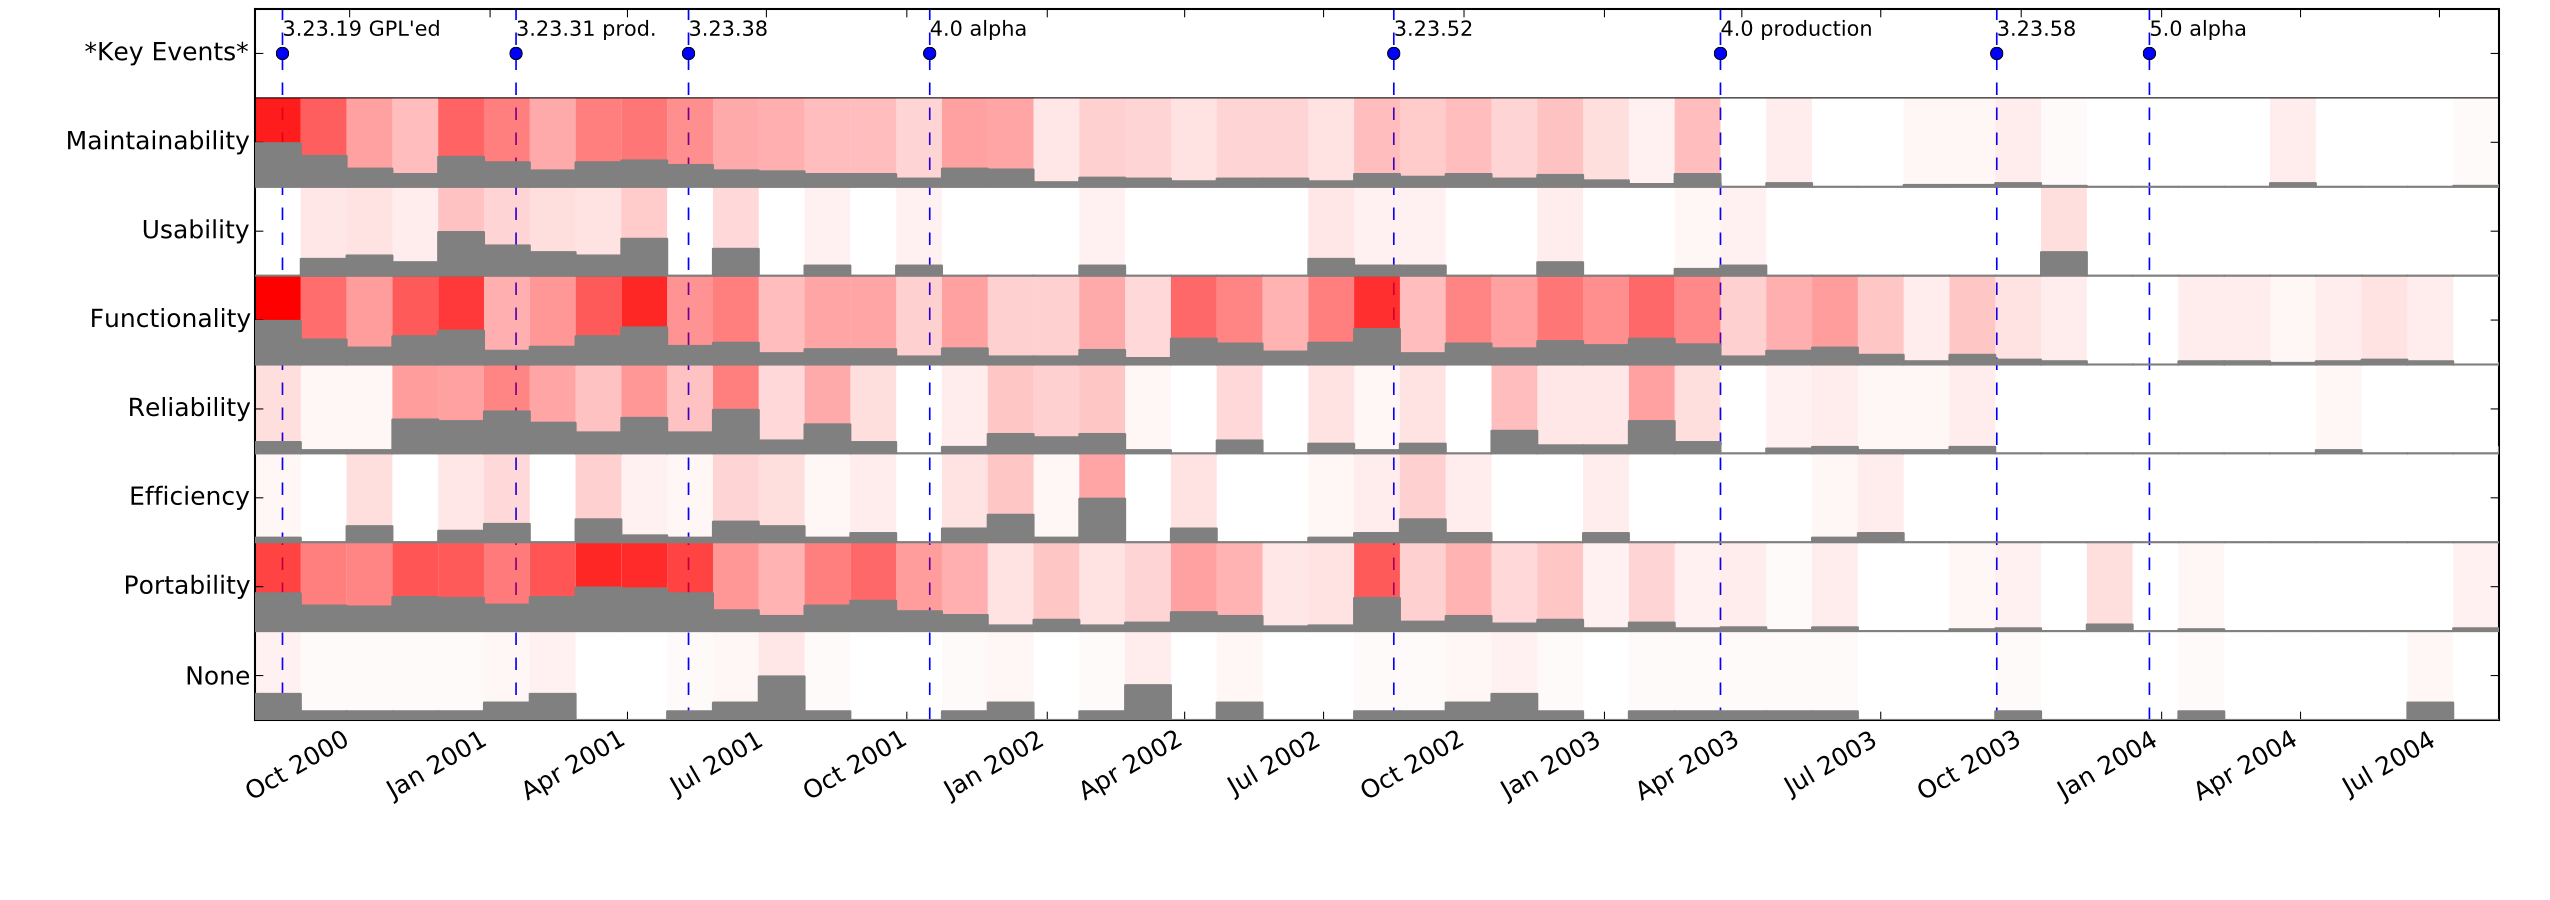
\includegraphics[width=\textwidth]{figures/mysql-timeline.png}
\label{fig:mysql-timeline}				 
}	    
					     
\subfloat[MaxDB 7.500]{					
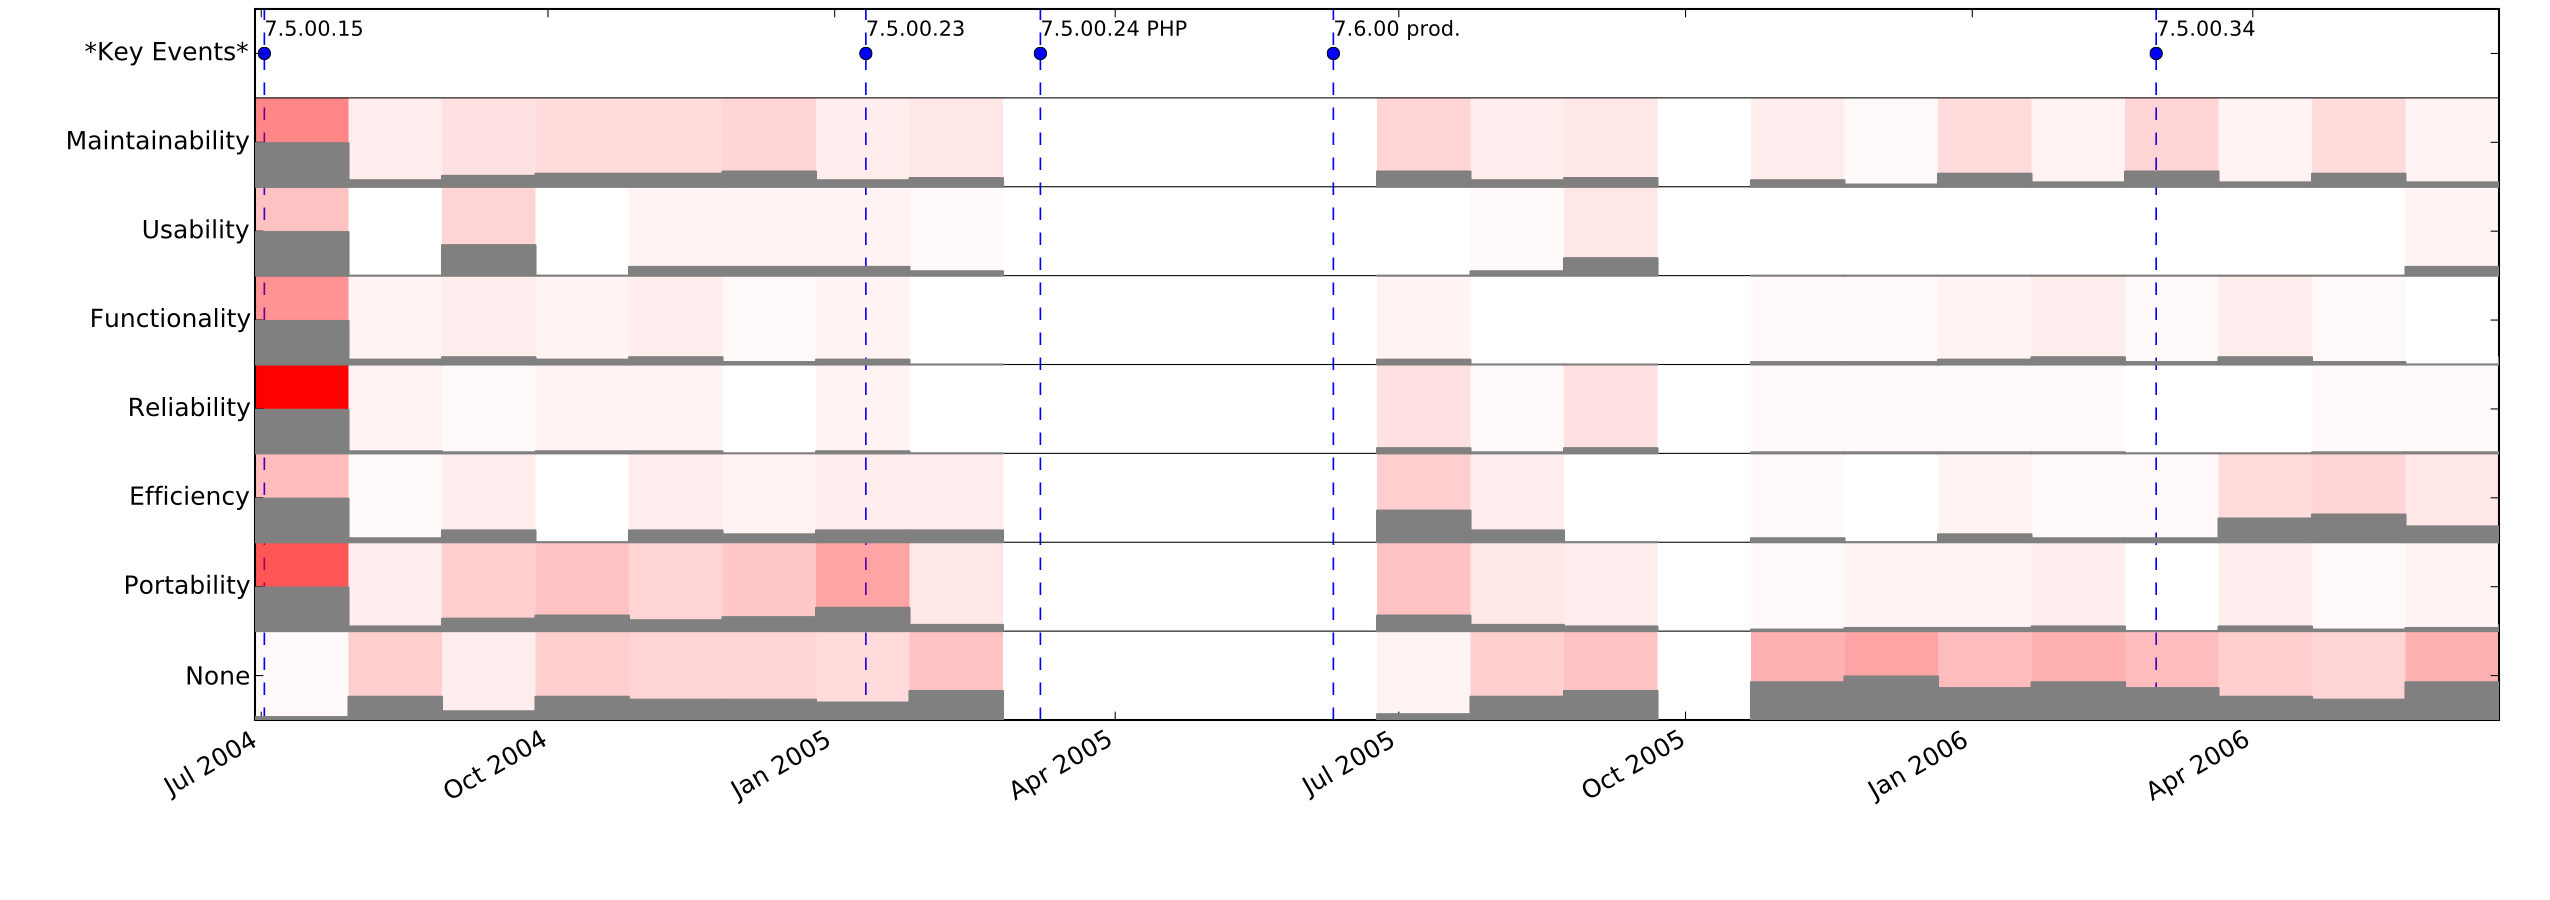
\includegraphics[width=\textwidth]{figures/maxdb-timeline.png}
\label{fig:maxdb-timeline}
}

\subfloat[PostgreSQL 7.2]{					
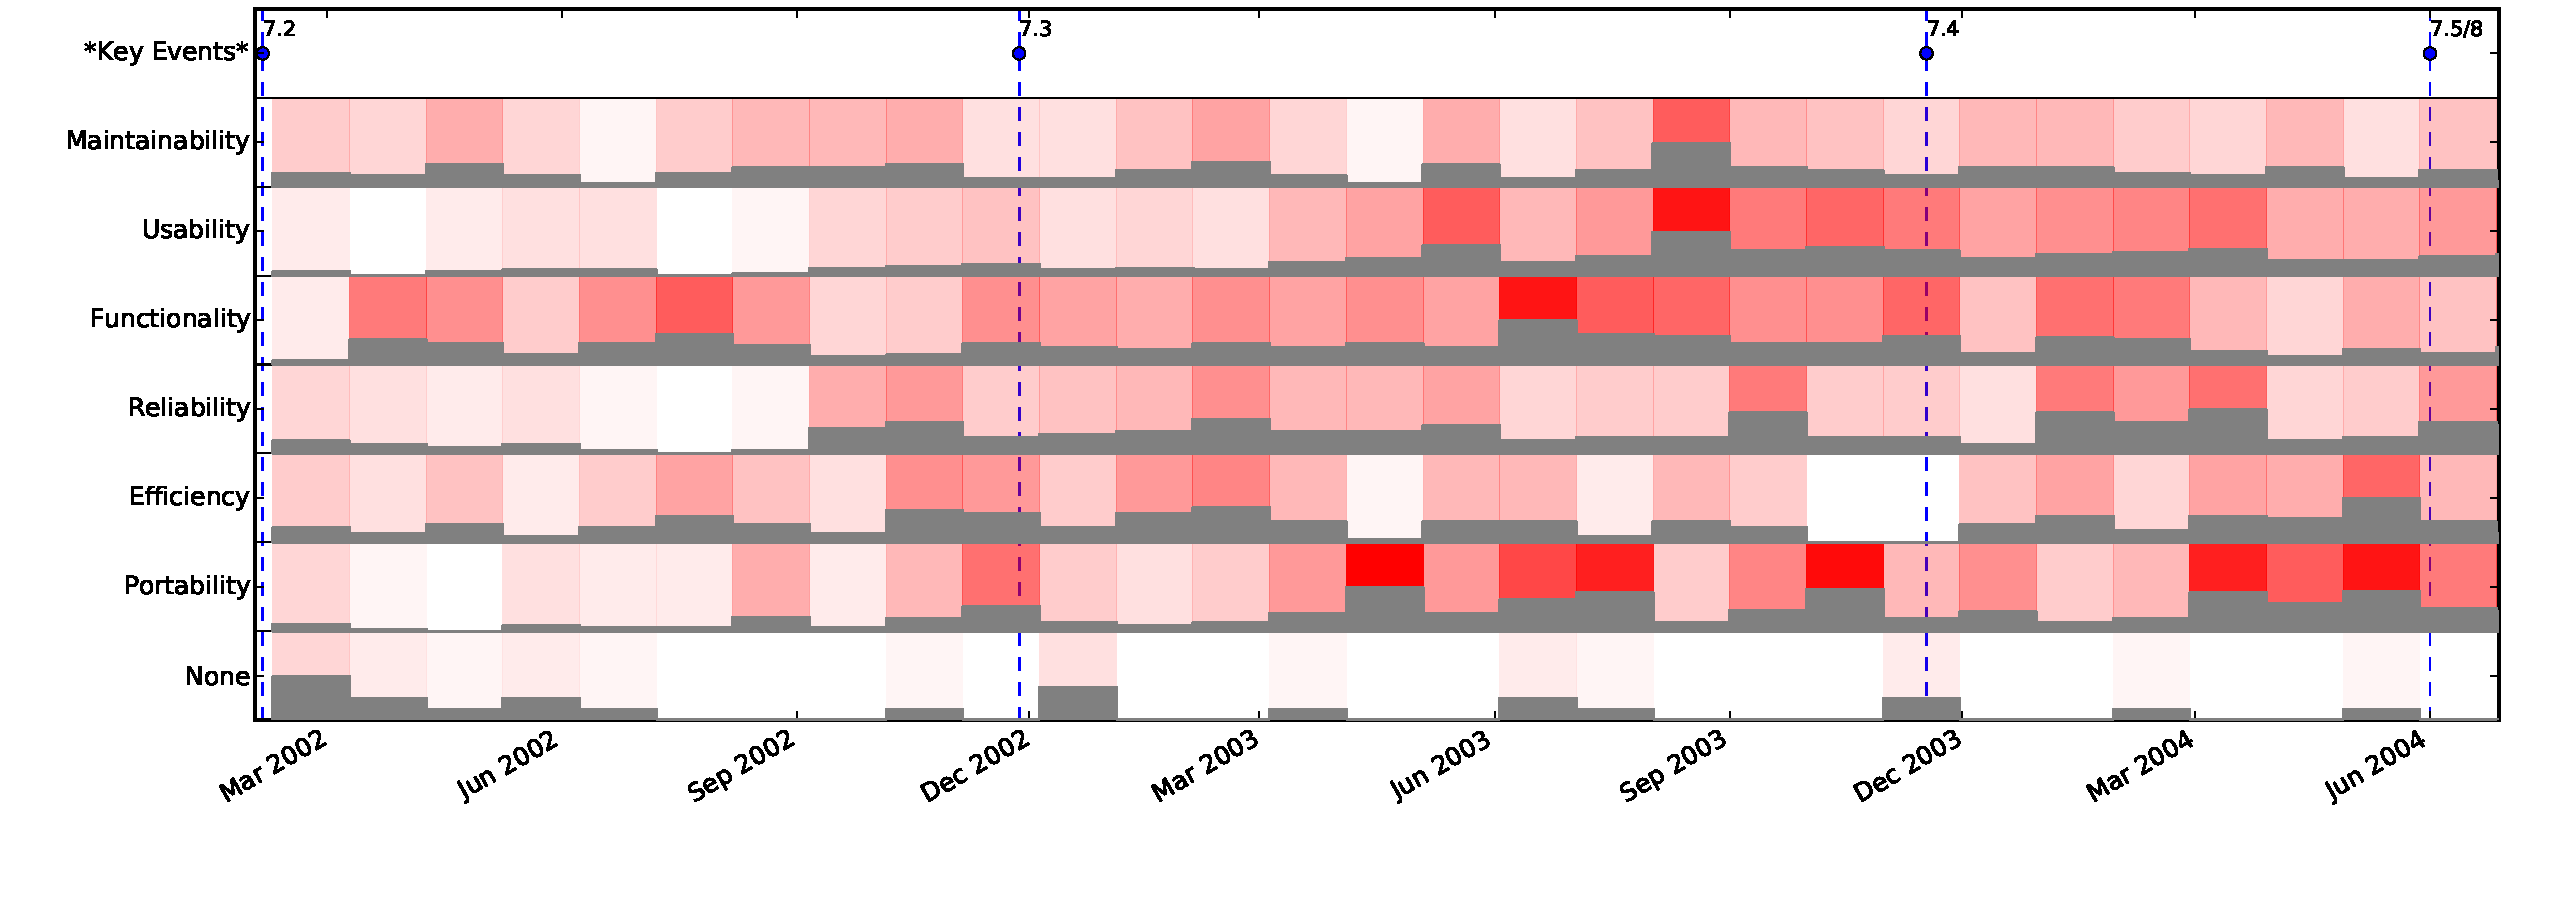
\includegraphics[width=\textwidth]{figures/pgsql-timeline}
\label{fig:pgsql-timeline}
}
	\caption[]{NFR label per period. Each cell represents a 30-day period. %Numbers represent number of topics in that period labelled with that NFR. 
	Grid cell intensity (saturation) is mapped to label frequency
	relative to the largest label count of \emph{all} NFRs. Grey
	histogram bars indicate label frequency relative to that
	particular NFR's largest label count. Dashed vertical lines
	relate a project milestone (\emph{*Key events*}) to our topic windows. 

}
\label{fig:timelines}
% Timelines created using src/validate/summary_labels.py
\end{figure}

%\noindent \textbf{Understanding the figures} -- 
 % boxes. not sure boxes is important..
% I grepped query1.mrs2 http://softwareprocess.es/y/y/maxdb-76.tar.gz
% and			http://softwareprocess.es/y/maxdb-7500.tar.gz
%There are more \textsf{None} labels in MaxDB because a number of topics were to do with code cleanup or automated checking using tools like
%\texttt{sutcheck}, a tool specific to the development process of MaxDB. 

%\noindent \textbf{Timeline of key events} -- 
We analyzed each project's developer mailing list for external validation. 
%As discussed earlier, the top row in each figure shows key events for each project. 
We use \textit{labelled topic extraction} to pick out the underlying NFR activity behind these events. 
For example, both MaxDB and MySQL show a high number of NFRs recognized at the first period of analysis. 
This is due to our window choice: we deliberately targeted our
analysis to when both MySQL 3.23
and MaxDB 7.500 were first announced. For MaxDB, version 7.5.00  was released in December of 2003. 
We know that release 7.5.00.23 saw the development of PHP interfaces, possibly accounting for the simultaneous increase in the \emph{portability}
NFR at the same time.
The gap in MaxDB (Figure \ref{fig:maxdb-timeline}) is due to a shift in development focus (from February 2005 to June 2005) to MaxDB 7.6, which is
released in June 2005.

%For MySQL (Figure \ref{fig:mysql-timeline}), we similarly validated our NFR patterns with external mailing list data. 
The release of MySQL we study  (Figure \ref{fig:mysql-timeline}) was the first to be licenced under the GPL. 
Version 3.23.31 (January, 2001) was the production release (non-beta), and we see a flurry of topics labelled with \emph{functionality} and
\emph{maintainability}. 
After this point, this version enters the maintenance phase of its life-cycle. 
In May 2001, there is an increase in the number of topics labelled with \emph{portability}. 
This might be related to release 3.23.38, which focused on Windows compatibility. 
Similarly, in August, 2002, both \emph{functionality} and \emph{portability} are frequent, and mailing list data suggests this is related to the release
of version 3.23.52, a general bug fix with a focus on security (a component of the \emph{functionality} NFR in the ISO9126 model). 
After this point, efforts shift to the newer releases (4.0, 4.1,
5.0). 

By contrast, the PostgreSQL timeline  (Figure \ref{fig:pgsql-timeline}) is extracted from a central trunk and is not version-specific. Therefore development 
tends to be focused on releases 7.3, 7.4 and 7.5/8.0 alpha. For example, a priority for the 8.0 candidate was a Windows-native port of the source code, which seems to 
correlate with the \emph{portability} NFR increasing in frequency in mid-2004. Before the 7.4 release, \emph{usability,functionality} and \emph{portability} all 
increase in frequency, possibly reflecting the interest in adding features and documentation for the release.

In the following sections we turn to our research questions:

% \subsection{Comparing MaxDB and MySQL}

% \label{sec:comparison}
%\XXX{Not sure there's enough here to do that!}
% We observed that MySQL had more topic subsets than MaxDB. 
% MySQL 3.23 also had more topics and a longer recorded history than MaxDB 7.500. 
% We tagged more MySQL topics with annotations than MaxDB topics, yet both shared similarities. 
% In terms of non-functional requirements both projects had long running trends that focused on \emph{functionality}, \emph{maintainability}, and
%\emph{portability}, yet MaxDB had more of a focus on \emph{efficiency} and \emph{reliability}. 
%\subsection{Research questions}
%This analysis allows to address the questions raised in Section \ref{sec:suplabelling}:
%This analysis addresses our research questions: %raised in Section \ref{sec:analysis}:

\subsection{Do NFR Frequencies Change over Time?}
%\noindent\textbf{1. Do NFR frequencies change over time?} --- 
%\subsubsection{Do label frequencies change over time?}

In both MaxDB and MySQL the frequencies generally decreased with age. 
However, there are variations within our NFR labels. In MySQL, \emph{usability} and \emph{efficiency} do not appear very often in topics. 
A proportionately smaller number of commits addressed these NFRs.
%As discussed in the previous section, 
Certain peaks in topic numbers coincide with a particular emphasis from the development team on issues such as new releases or bug fixes.
This suggests that maintenance activity is not necessarily strictly decreasing with time, but rather episodic and responsive to outside stimuli. 
In MaxDB, we can observe that \emph{Maintainability} topics became more prevalent as MaxDB matures. 
This is likely due to our analysis time-frame for MaxDB being shorter than the time-frame for the MySQL product. 

In PostgreSQL, by comparison, the frequencies seem to by cyclic, since we are not studying a maintenance-phase for the product, but rather ongoing
feature addition and usability improvements.

\subsection{Do Projects Differ in their Relative  Topic Interest?}
Yes. MySQL 3.23 had proportionally more
topics labelled \emph{functionality}, while MaxDB had proportionally more
\emph{efficiency} related topics. MaxDB was a very mature release ``donated'' to the open-source community, 
whereas MySQL was in its relative infancy, and	
security problems were more common (security is a component of \emph{functionality} in the ISO9126 model). 
In both cases \emph{portability} was a constant maintenance concern and was prevalent throughout the lifetime of the projects. It may surprise developers
how often portability arises as a concern.
\todo{add the pgsql data}

\subsection{Do different developers work on different NFRs?}

%data/clusters.R

We wanted to see how similar developers were to each other in terms of
the NFRs that worked on. First we did pairwise $X^2$ (chi-squared)
tests and Kolmogorov-Smirnov tests for each developer pair and we
found that $3/10$ of these tests the developers were significantly
different, that is their distributions were not similar. This implies
that there are authors who focus on different NFRs or different
proportion of NFRs.

In Figure \ref{fig:authorcluster} we clustered developers using the
Ward method of Hierarchical clustering.  This diagram shows that
\texttt{petere}, \texttt{tgl} and \texttt{momjian} form their own
cluster (they are also the most frequent committers). This is
interesting because it means that the important developers are not
committing code that fits the same NFR profile. In terms of the larger
cluster we can see that \texttt{momjian} and \texttt{tgl} are in the
same cluster, but \texttt{petere} is not. The most frequent
committers do not share the same clusters. This implies that
developers do work on different sets of NFRs and have different
software quality focus.

Figure \ref{fig:authorcluster} clustered the authors into $2$ clusters
and $6$ clusters. We chose $6$ because the difference in width between
entities and centroids was minimal at $6$ and the derivative of was
the highest in that region as well.

It should be noted that much of PostgreSQL development originates from
the mailinglist and the developers are often pushing integrations. If
we compare the total to each author we find that 1 quarter of the
authors have a similarity of $0.47$ or less. This is depicted in
Figure \ref{fig:authorsim} where we can see that not all authors are
as similar to the global trend as others. Of
course, we found that number of commits had a strong correlation
($0.59$ Pearson) between the similarity to the aggregate and the
number of topics associated with that author.

Our theory is that the less frequent committers are more
focused and less general, thus their distributions of topics are
different than the main developers who commit code in many different
contexts.  The lead developers either ``wear more hats'' or have more
time to ``wear more hats''.

Given the top 15 PostgreSQL devs we found that proportionally many
devs had a focus on NFR topics. Authors with top proporitions per NFR
were:
\texttt{dennis} for usability; 
\texttt{scrappy} and \texttt{meskes} for portability;
\texttt{inoue} and \texttt{neilc} for efficiency;
\texttt{jurka} and \texttt{joe} for reliability;
\texttt{thomas} and \texttt{weick} for functionality;
and \texttt{ishii} and \texttt{scrappy} for maintainability.
Given these results we found that yes indeed there was often a focus
of $1/3$ to $1/10$ of commits dedicated to a particular NFR.


% Dennis is into usability
% scrappy and meskes portability
% Inoue and neilc for effiency
% jurka joe and barry for Reliabilityb
% thomas weick teodor for Functionality
% ishii, scrappy, darcy for maintainability

%\todo{Now look at the authors, what are they into?}

% tgl == momjian
% > nauthors
%                     momjian     thomas      davec      neilc      ishii darcy
% None            0.003       0.150       0.048       0.020       0.081       0.15
% Portability     0.211       0.083       0.177       0.173       0.122       0.20
% Efficiency      0.114       0.100       0.080       0.152       0.132       0.00
% Reliability     0.149       0.100       0.137       0.159       0.102       0.15
% Functionality   0.220       0.300       0.266       0.145       0.214       0.20
% Maintainability 0.132       0.150       0.145       0.104       0.224       0.20
% Usability       0.167       0.116       0.145       0.243       0.122       0.10
%                      barry      wieck      inoue      pgsql teodor jurka
% None            0.03488372 0.04444444 0.04166667 0.06521739 0.0250  0.04
% Portability     0.13372093 0.17777778 0.09722222 0.19565217 0.2250  0.18
% Efficiency      0.13372093 0.08888889 0.26388889 0.15217391 0.1250  0.12
% Reliability     0.19767442 0.11111111 0.12500000 0.06521739 0.0875  0.24
% Functionality   0.20930233 0.28888889 0.23611111 0.19565217 0.2375  0.16
% Maintainability 0.13372093 0.06666667 0.13888889 0.17391304 0.1250  0.14
% Usability       0.15697674 0.22222222 0.09722222 0.15217391 0.1750  0.12
%                         tgl    scrappy     petere     dennis     meskes
% None            0.006704981 0.08333333 0.02296451 0.06451613 0.02298851
% Portability     0.207854406 0.25000000 0.20250522 0.22580645 0.23754789
% Efficiency      0.119731801 0.08333333 0.09812109 0.12903226 0.08045977
% Reliability     0.150383142 0.16666667 0.12734864 0.09677419 0.14559387
% Functionality   0.217432950 0.12500000 0.20668058 0.12903226 0.22222222
% Maintainability 0.129310345 0.20833333 0.14196242 0.00000000 0.10727969
% Usability       0.168582375 0.08333333 0.20041754 0.35483871 0.18390805
%                        joe
% None            0.06122449
% Portability     0.22448980
% Efficiency      0.08163265
% Reliability     0.22448980
% Functionality   0.12244898
% Maintainability 0.10204082
% Usability       0.18367347


\begin{figure}
  \centering
  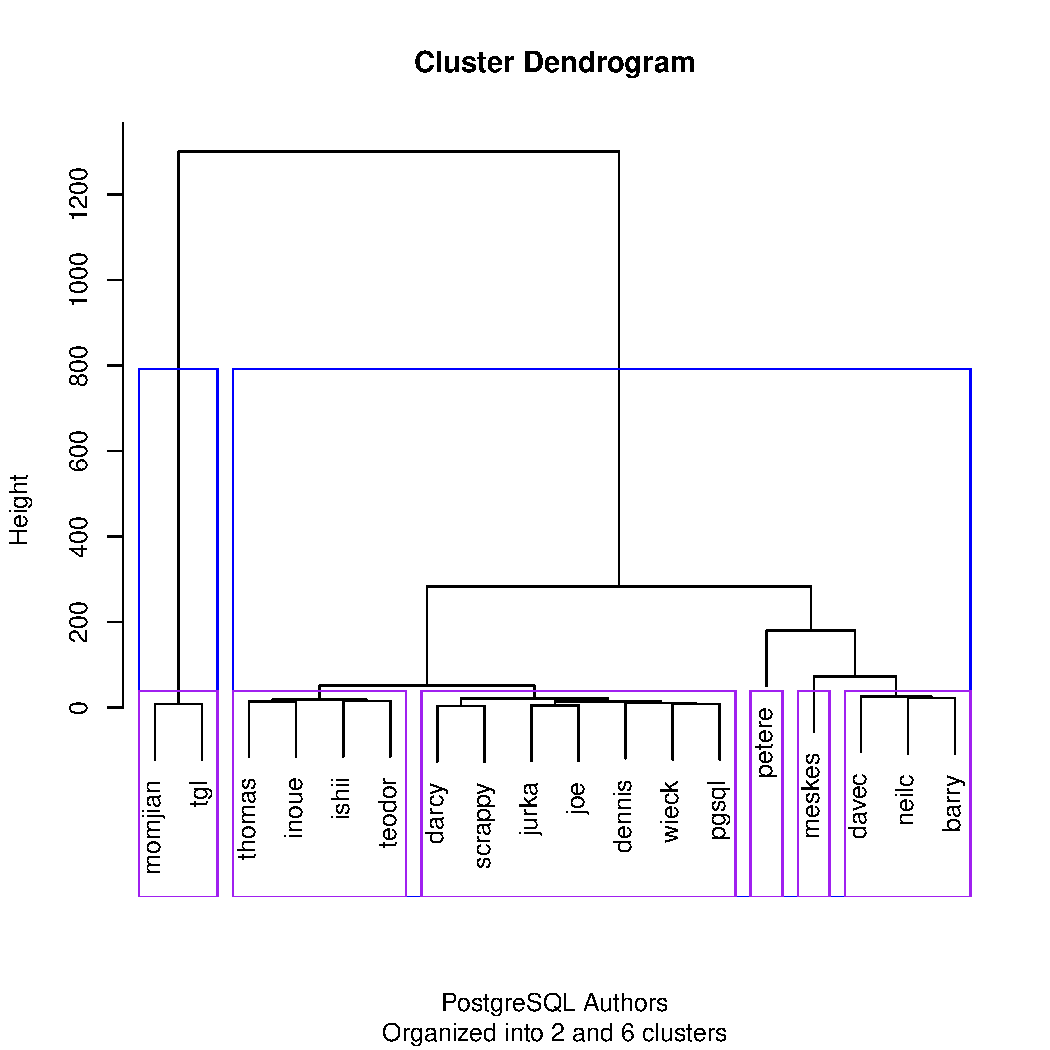
\includegraphics[width=.9\textwidth]{figures/postgresql-author-cluster}
  \caption{PostgreSQL Author Clusters: Authors clustered by cosine
    distance of their NFR contributions}
\label{fig:authorcluster}
\end{figure}




\begin{figure}
  \centering
  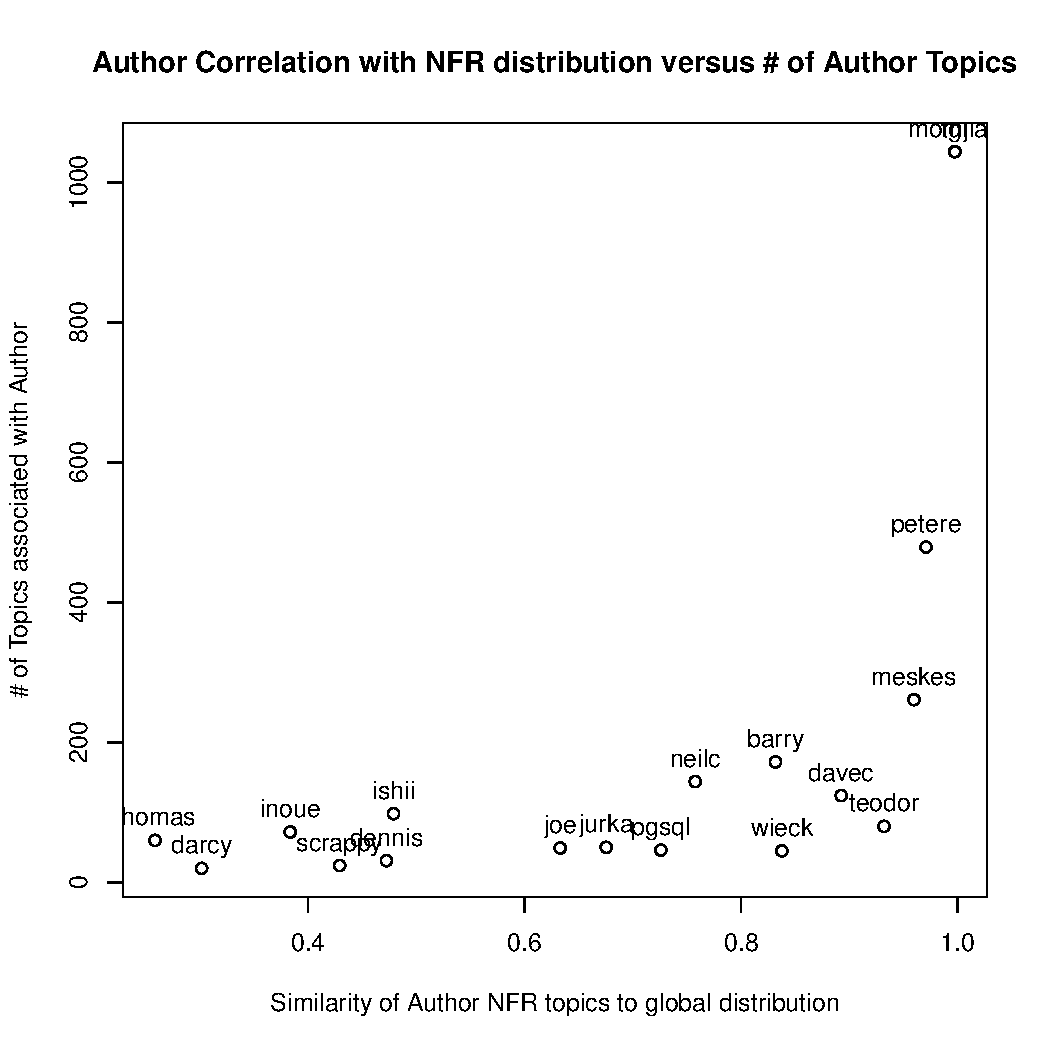
\includegraphics[width=.9\textwidth]{figures/author-distance-from-aggregate}
  \caption{PostgreSQL Author Similarity to the Global Distribution of NFR topics}
\label{fig:authorsim}
\end{figure}


\section{Discussion}
\label{sec:limit}

\subsection{Annotation Observations}
We found many topics that were not actually non-functional requirements (NFRs) but were often related to them. 
For instance, concurrency was mentioned often in the commit logs and
was related to \emph{correctness} and \emph{reliability}, possibly because concurrent code is prone to bugs such as race conditions. %are 
% often  was troublesome. 
\emph{Configuration management} and \emph{source control} related changes appeared often; % and sometimes there were topics dedicated to configuration
management. 
these kinds of changes are slightly related to \emph{maintainability}. 
A non-functional change that was not quality-related was licensing and
copyright; many changes were simply to do with updating copyrights or
ensuring copyright or license headers were applied to files. In these
cases we assigned the \emph{None} label to the topic.

We noticed that occasionally the names of modules would conflict with words related to other non-functional requirements. 
For instance, optimizers are very common modules in database systems: both MySQL and MaxDB have optimizer modules. 
In MySQL the optimizer is mentioned but often the change addresses  correctness or another quality. 
Despite this difference, the name of the module could fool our learners into believing the change was always about \emph{efficiency}. 
In these cases the advantages of tailoring topic names to specific project terminologies are more clear. 
Project specific word-lists would avoid automated mistakes due to the names of entities and modules of a software project.

\subsection{Inter-rater reliability}

To determine inter-rater reliability two of the authors---Ernst and Hindle---each annotated the PostgreSQL topics,
and then evaluated each other's annotations.

%>    A_portability   A_functionality     A_reliability A_maintainability
%>      0.153548387      -0.013588517       0.004573794       0.082001031
%>     A_efficiency       A_usability            A_none
%>      0.231496539       0.009287926       0.062133646

% > Spearman says
% >   A_portability   A_functionality     A_reliability A_maintainability
% >      0.253037469      -0.014415214       0.004579664       0.082215613
% >     A_efficiency       A_usability            A_none
% >      0.258037216       0.014436230       0.080667468

\begin{table}
\centering
\begin{tabular}{l|c|c}
\hline
            & Cohen's Kappa & Spearman Correlation \\ \hline
Portability & 0.154 & 0.253  \\
Functionality & -0.014 & -0.014 \\
Reliability & 0.005 & 0.005 \\
Maintainability & 0.082 & 0.082 \\
Efficiency & 0.231 & 0.258 \\
Usability & 0.009 & 0.014 \\
None &      0.062 & 0.081 \\ \hline 
Everything & 0.107 & 0.108 \\ \hline
\end{tabular}
\caption{Inter-rater Reliability on PostgreSQL}
\label{tab:interr}
\end{table}

Table \ref{tab:interr} describes the Cohen Kappa and the Spearman
correlation of our per topic annotations for each tag. We had to
evaluate inter-rater reliability this way because 1 topic could be
tagged with more than 1 annotation.

We feel these results are poor. The aggregate view of with a Kappa of
$0.1$ indicates there is some agreement but not a lot. We found that
there was a lot of agreement in terms of lack of a tag, but often more
disagreement when a tag should be applied.

After some discussion we concluded that usability was a source of
disagreement. Do user manuals improve usability? Is a command-line
option a usability issue? These kinds of questions illustrate some of
the agreement, disagreement and ambiguity about these labels. Furthermore, 
both annotators found that the annotation was time-consuming and
difficult.

% I think this is largely due to lack of training. So I will write it up as such - as an interesting point to say that agreeing on the meaning of "software quality" is difficult, etc. Ideally we would now do a sample training session where we go over say one period and determine the appropriate annotations, then recalculate Kappa to see what changes.

% The other tack is to ignore the IRR data completely as we did in the workshop. But I don't think it hurts our results that much ¦ just confirms the difficulty of annotation.

% Neil



\subsection{Summary of Techniques}
While an unsupervised technique such as LDA is appealing in its lack of human intervention, and thus lower effort, 
supervised learners have the advantage of domain knowledge, which typically means improved results. 
% NEIL - we got criticized for making it sound like this is the obvious thing to do... and then why do you need a learner?
%Our manual annotations were fairly quick to do, taking only a few minutes per 30 day period. 
Creating annotated topics (i.e., manual labels) for training is painstaking, but with a suitably representative set of topics, the effort is acceptable. To
annotate \emph{all} topics took us approximately 20 hours per project, but we estimate only 10\% of the topics need annotation to produce useful results.

Very rarely did \textsf{exp2} and \textsf{exp3} (semi-unsupervised word matching) ever perform as well as the supervised machine learners. 
For MaxDB, \textit{reliability} was slightly better detected using the static word list of \textsf{exp2}. 
In general, the machine learners and \textsf{exp3} did better than \textsf{exp2} for both MaxDB and MySQL. 
For both MySQL and MaxDB \textit{usability} was better served by \textsf{exp2}. 
\textit{Usability} was a very infrequent label, however, which made it difficult to detect in any case.

The semi-unsupervised labelling had difficulty distinguishing between common labels and infrequent labels. 
The learners would occasionally mislabel a topic deserving of an infrequent label with a more common label.
The word-lists for \emph{correctness} tended to be too lengthy, non-specific and broad, especially if WordNet words were used, since the NFRs are
typically loosely defined concepts in common parlance.

We found that the multi-label learners of BR, CLR and HOMER only did
as well or worse for Macro-ROC as the single-label Naive Bayes and other naive Bayes-derived learners. 
This suggests that by combining together multiple Naive Bayes learners
we could probably label sets of topics effectively, but it would
require a separate Naive Bayes learner per label.

%{Discuss how these are CHEAP techniques and although somewhat %inaccurate they don't require a tonne of work}

With ROC values ranging from $0.6$ to $0.8$ we can see there is promise in these methods.
\textsf{exp2} and \textsf{exp3} both indicate that static information can be used to help label topics without any training whatsoever. 
MySQL and MaxDB's machine learners made some decisions based off a few shared words: \textsf{bug, code, compiler, database, HP UX, delete, memory,
missing, problems, removed, add, added, changed, problem, and test}. 
Adding these words to the word-lists of \textsf{exp2} and \textsf{exp3} could improve performance while ensuring they were only domain specific.

If the techniques used in \textsf{exp2} and \textsf{exp3} were combined with the supervised techniques, we could reduce the training effort by boosting
training sets with topics classified with the semi-unsupervised techniques.
Both Naive Bayesian learners and the word-list approaches were computationally efficient.  
%These results are promising, because the accuracy of the techniques is good enough to be useful, while the run-time performance is still cheap enough
%to execute to be feasible as an automated or semi-automated method of labelling topics by their software qualities.
These results are promising because they indicate that these
techniques are accurate enough to be useful while still maintaining
acceptable run-time performance.

Since this work focuses on labelling natural language commit log
comments we feel it can be adapted to other natural language artifacts
such as mailing-list discussions and bug reports, even though that was
not evaluated in this paper. Bug reports might not exhibit the same
behaviour as commits in terms of dominant topics.

\subsection{Threats to Validity}
% can always be cut down
%Our work faced multiple threats to validity and we attempted to address many of them.
\emph{Construct validity} -- we used only commit messages rather than
mail or bug tracker messages. 
To extend further we would need matching repositories for each project.
%Each case study was BecauseSince we required a seamless record, it was not possible to obtain
%other data sources. 
Possibly they would have influenced our results, but there would be a degree of correlation between the corpora.
%Conversely, construct validity was addressed in our validation as we used the files, topics and revisions to annotate the commit messages. 
%We used mailing-lists to verify the purpose behind some events.
Our taxonomy for software NFRs is subject to dispute, but seems
generally accepted. Finally, there are exogenous sources, such as
in-person discussions, which we did not access, an omission as noted
in Aranda et al.~\cite{aranda09icse} %We did not show these results to the stakeholders.

\emph{Internal validity} -- %includes inter-rater reliability and our lack of rival explanation building. 
We improved internal validity by trying to correlate and explain the behaviours observed in the analysis with the historical records of the projects.
We did not attempt to match our results to any particular model.
We assessed inter-rater reliability (IRR), a measure of the correlation between the manual annotations the first two authors created. Perfect IRR (1.0) indicates complete agreement 
on the appropriate annotation for that topic. We verified IRR using
manually annotated PostgreSQL topics, and achieved a result of $0.1$.
Some of the reasons for this are a disagreement over the appropriate classification for documentation topics (should this be considered
usability or portability?). A short education session on what a given NFR from the ISO standard encompasses would reduce this error rate.

\emph{External validity} -- %was addressed by our use of two case studies, but there are still issues. 
Our data originated from OSS database projects and thus might not be applicable to commercially developed software or other domains. 
Furthermore, our analysis techniques rely on a project's use of meaningful commit messages, although we feel this is the most frequently occurring form
of developer comments. 
%The OSS projects investigated were database systems, thus 
%our results might not generalize to other domains. %We only studied database systems.


% in Case Study Research: Design Case Studies
\emph{Reliability} -- each annotator, the first two authors, followed the same protocol and used the same annotations. 
However, only two annotators were used; their annotations could be
biased as we did not analyze for inter-rater reliability because they
did not rate the same documents.

\subsection{Future Work}
There are several avenues of further investigation.  
More external validation would be useful. 
Although we validated our comparisons using a mailing list for each project, interviews with developers would provide more detail. 
We also think multi-label learning techniques, although in their infancy, are crucial in understanding cross-cutting concerns such as NFRs. 
We want to leverage different kinds of artifacts to discover threads of NFR-related discussions that occur between multiple kinds of artifacts.
Finally, we would like to extend this analysis to other domains, to see what patterns might occur in, for example, a consumer-facing software product.

\section{Conclusions}
This paper presented a cross-project data mining technique,
\emph{labelled topic extraction}. %The technique leveraged a
%non-functional requirements (NFRs) taxonomy to mine and label latent
%software development topics. 
Previous topic analysis research produced project-specific
topics that needed to be manually labelled.
%, but topics without labels
%are difficult to interpret, and manually labelling them is
%costly. Furthermore, previous work was project-specific and thus incomparable. 
To improve on this, we leveraged software engineering standards,
specifically the ISO9126 quality taxonomy, to produce a method of partially-automated (supervised) and fully-automated (semi-unsupervised) topic labelling.
Since the word-list technique is not project-specific, we used it to compare three distinct projects, where we showed our technique produced interesting
insight into maintenance activity. %topics and artifacts from project histories.
% Our contributions include:
% \begin{itemize}
% \item We provided an unsupervised method of topic labelling (word-lists);
% %\item Our unsupervised method can be applied to projects without training;
% \item We demonstrated a supervised method of labelling topics by a single NFRs (machine learning);
% \item We demonstrated a supervised method of labelling topics by multiple NFRs (multi-label machine learning);
% \item We provided a method of cross-project analysis via topic labelling;
% \item We demonstrated a method of visualizing these topics across time, which we used to analyze maintenance activities.
% \end{itemize}


We validated our topic labelling techniques using multiple experiments. % on unsupervised learners, supervised and multi-label learners. 
We first conducted semi-unsupervised labelling using word-lists. 
Our next approach was supervised, using single-label and multi-label learners. 
Both kinds of learners performed well with average
%area under the 
ROC values between $0.6$ and $0.8$. These results, along with the efficient performance of our learners, demonstrate that labelled topic extraction is
a promising approach for understanding the occurrence of non-functional requirements in software projects. 
%Although it may seem like common knowledge that maintenance is a concern as a project matures, our technique was able to show this independently.
%We showed that NFRs are often trending topics in commit comments
%, and that NFRs are quite common as developer topics.
%; and that there are efficient methods of automating topic labelling.

%%%HMMM

Our data and scripts are available at:

\url{http://softwareprocess.es/nomen/}

% We demonstrated multiple supervised and unsupervised methods of topic labelling, including multi-label learners.
% We provided a case study and visualization of NFR related topics in MaxDB 7.500 and MySQL 3.23. 
% During the case study we manually labelled hundreds of topics by hand and then used these annotations to validate the positive performance of topic
%labelling techniques.
% The implication of our paper is that topics with labels are more useful for analyzing software development activities than are unlabelled topics. To
%furnish stakeholders with labelled topics, our technique provides many methods of automatic topic labelling.


%\begin{acknowledgements}
%\end{acknowledgements}

% BibTeX users please use one of
%\bibliographystyle{spbasic}	  % basic style, author-year citations
\bibliographystyle{spmpsci}	 % mathematics and physical sciences
%\bibliographystyle{spphys}	  % APS-like style for physics
\bibliography{ese}   % name your BibTeX data base

\end{document}
% end of file template.tex

